	%% LLT: Turn off some annoying warnings...
\RequirePackage{silence}
\WarningFilter{titlesec}{Non standard sectioning command}
\WarningFilter{scrreprt}{Usage of package}
\WarningFilter{scrreprt}{Activating an ugly workaround}
% **************************************************
% Document Class Definition
% **************************************************
\documentclass[					%
	paper=A4,					% paper size --> A4 is default in Germany
%	twoside=true,				% onesite or twoside printing
    oneside=true,
%	twoside=false,				% onesite or twoside printing
	openright,					% doublepage cleaning ends up right side
	parskip=full,				% spacing value / method for paragraphs
	chapterprefix=true,			% prefix for chapter marks
	10pt,						% font size
	headings=small,				% size of headings		
%	bibliography=totoc,			% include bib in toc
%	listof=totoc,				% include listof entries in toc
	titlepage=on,				% own page for each title page
	captions=tableabove,			% display table captions above the float env
	draft=false, 				% value for draft version
]{scrreprt}						%

\usepackage{csvsimple,longtable,booktabs}
\usepackage{tocloft}
\usepackage{graphicx}				% Grafiken
\usepackage[utf8]{inputenc}			% defines file's character encoding
\usepackage{paralist}          		% for compactitem itemization
\usepackage{chngcntr}           		% Einfache Nummerierung von Abbildungen
\counterwithout{figure}{chapter} 	% Einfache Nummerierung von Abbildungen
\usepackage{listings} 				% Code Listings
\usepackage{float} 					% exaktes Figure Placement mit H
\usepackage[center]{caption}          		% Figure-Captions formatieren
\usepackage[table,xcdraw]{xcolor}
\usepackage[german,ruled]{algorithm2e}

% change font-size algorithm2e
\SetAlFnt{\footnotesize}
\SetAlgoLined

\lstset{
  breaklines=true,
%  numbers=left,
  numbersep=5pt,
  basicstyle=\footnotesize\ttfamily,
  numberstyle=\tiny\color{black}
%  literate=%
%  {Ö}{{\"O}}1
%  {Ä}{{\"A}}1
%  {Ü}{{\"U}}1
%  {ß}{{\ss}}2
%  {ü}{{\"u}}1
%  {ä}{{\"a}}1
%  {ö}{{\"o}}1
}
\lstset{literate=
  {á}{{\'a}}1 {é}{{\'e}}1 {í}{{\'i}}1 {ó}{{\'o}}1 {ú}{{\'u}}1
  {Á}{{\'A}}1 {É}{{\'E}}1 {Í}{{\'I}}1 {Ó}{{\'O}}1 {Ú}{{\'U}}1
  {à}{{\`a}}1 {è}{{\`e}}1 {ì}{{\`i}}1 {ò}{{\`o}}1 {ù}{{\`u}}1
  {À}{{\`A}}1 {È}{{\'E}}1 {Ì}{{\`I}}1 {Ò}{{\`O}}1 {Ù}{{\`U}}1
  {ä}{{\"a}}1 {ë}{{\"e}}1 {ï}{{\"i}}1 {ö}{{\"o}}1 {ü}{{\"u}}1
  {Ä}{{\"A}}1 {Ë}{{\"E}}1 {Ï}{{\"I}}1 {Ö}{{\"O}}1 {Ü}{{\"U}}1
  {â}{{\^a}}1 {ê}{{\^e}}1 {î}{{\^i}}1 {ô}{{\^o}}1 {û}{{\^u}}1
  {Â}{{\^A}}1 {Ê}{{\^E}}1 {Î}{{\^I}}1 {Ô}{{\^O}}1 {Û}{{\^U}}1
  {œ}{{\oe}}1 {Œ}{{\OE}}1 {æ}{{\ae}}1 {Æ}{{\AE}}1 {ß}{{\ss}}1
  {ű}{{\H{u}}}1 {Ű}{{\H{U}}}1 {ő}{{\H{o}}}1 {Ő}{{\H{O}}}1
  {ç}{{\c c}}1 {Ç}{{\c C}}1 {ø}{{\o}}1 {å}{{\r a}}1 {Å}{{\r A}}1
  {€}{{\EUR}}1 {£}{{\pounds}}1
}

\usepackage{minted} % needed for the inclusion of source code
\usepackage{pgfplots} % needed for drawing diagrams
\usepackage{pgfplotstable}
\usetikzlibrary{matrix}
\usepackage{textcomp}
\usepackage{amsmath}
\usepackage{amssymb}
\usepackage{mathtools} 
\usepackage{array}
\usepackage{color}
\usepackage{colortbl}
\usepackage{multirow}
\usepackage{hhline}
\usepackage{filecontents} 
% **************************************************
% Information and Commands for Reuse
% **************************************************
\newcommand{\thesisTitle}{Bachelorarbeit}
\newcommand{\thesisName}{Lukas Abegg}
\newcommand{\thesisMatrikelNr}{Matrikelnummer 798972}
\newcommand{\thesisSubtitle}{Suchoptimierung mittels maschinellen Lernens}
\newcommand{\thesisZeitraum}{Zeitraum 04.07.2016 - 11.10.2016}
\newcommand{\thesisSemester}{Sommersemester 2016}
\newcommand{\thesisDate}{Oktober 11, 2016}

\newcommand{\thesisFirstReviewer}{Prof. Dr. habil. Alexander Löser}
\newcommand{\thesisFirstPosition}{Fachbereich VI - Informatik und Medien}
\newcommand{\thesisFirstReviewerUniversity}{\protect{Beuth Hochschule f{\"u}r Technik}}
\newcommand{\thesisFirstReviewerUniversitySmall}{\protect{Beuth Hochschule}}
\newcommand{\thesisFirstReviewerUniversityCity}{Berlin}
\newcommand{\thesisFirstReviewerUniversityStreetAddress}{Luxemburger Str. 10}
\newcommand{\thesisFirstReviewerUniversityPostalCode}{13353}

\newcommand{\thesisSecondReviewer}{Prof. Dr. rer. nat. Elmar Böhler}
\newcommand{\thesisSecondPosition}{Fachbereich VI - Informatik und Medien}
\newcommand{\thesisSecondReviewerUniversity}{\protect{Beuth Hochschule f{\"u}r Technik}}
\newcommand{\thesisSecondReviewerUniversitySmall}{\protect{Beuth Hochschule}}
\newcommand{\thesisSecondReviewerUniversityCity}{Berlin}
\newcommand{\thesisSecondReviewerUniversityStreetAddress}{Luxemburger Str. 10}
\newcommand{\thesisSecondReviewerUniversityPostalCode}{13353}

\newcommand{\thesisUniversity}{\protect{Beuth Hochschule f{\"u}r Technik}}
\newcommand{\thesisUniversityDepartment}{Studiengang Medieninformatik (B.Sc.)}
\newcommand{\thesisFachsemester}{Fachsemester 6}
\newcommand{\thesisUniversityCity}{Berlin}
\newcommand{\thesisUniversityStreetAddress}{Luxemburger Str. 10}
\newcommand{\thesisUniversityPostalCode}{13353}

% **************************************************
% Debug LaTeX Information
% **************************************************
%\listfiles

% **************************************************
% Load and Configure Packages
% **************************************************
\usepackage[german]{babel}    		% Deutsche Sprache in automatisch generiertem
\usepackage[							% use bachelorthesis style
	figuresep=colon,%
	sansserif=false,%
	hangfigurecaption=false,%
	hangsection=false,%
	hangsubsection=false,%
	colorize=full,%
	colortheme=bluemagenta,%
	bibsys=bibtex,%
	bibfile=bib-refs,%
	bibstyle=alphabetic,	%
]{bachelorthesis}

\hypersetup{								% setup the hyperref-package options
	pdftitle={\thesisTitle},				% 	- title (PDF meta)
	pdfsubject={\thesisSubtitle},		% 	- subject (PDF meta)
	pdfauthor={\thesisName},				% 	- author (PDF meta)
	plainpages=false,					% 	-
	colorlinks=false,					% 	- colorize links?
	pdfborder={0 0 0},					% 	-
	breaklinks=true,						% 	- allow line break inside links
	bookmarksnumbered=true,				%
	bookmarksopen=true					%
}

\sloppy


% **************************************************
% Document CONTENT
% **************************************************
\begin{document}

\setstretch{1.1}
 
% --------------------------
% rename document parts
% --------------------------
\renewcaptionname{german}{\figurename}{Abb.}
\renewcaptionname{german}{\tablename}{Tab.}
\renewcommand\listingscaption{Code}
\renewcommand\listoflistingscaption{Sourcecode-Verzeichnis}
\renewcaptionname{german}{\listfigurename}{Abbildungs-Verzeichnis}
\renewcaptionname{german}{\listtablename}{Tabellen-Verzeichnis}
\renewcommand{\cftlottitlefont}{\color{ctcolorblack}\huge \fontfamily{phv}\selectfont}
\renewcommand{\cftloftitlefont}{\color{ctcolorblack}\huge \fontfamily{phv}\selectfont}

% --------------------------
% Formulas
% --------------------------
\setlength{\abovedisplayskip}{0pt}
\setlength{\abovedisplayshortskip}{0pt}
\setlength{\belowdisplayskip}{0pt}
\setlength{\belowdisplayshortskip}{0pt}
    
% --------------------------
% itemize
% --------------------------
\newenvironment{myitemize}
{ \begin{itemize}
    \setlength{\itemsep}{0pt}
    \setlength{\parskip}{0pt}
    \setlength{\parsep}{0pt}     }
{ \end{itemize}                  } 

% --------------------------
% Front matter
% --------------------------
\pagenumbering{roman}				% roman page numbing (invisible for empty page style)
\pagestyle{empty}					% no header or footers
% ------------------------------------  --> cover title page
\begin{titlepage}
	\pdfbookmark[0]{Cover}{Cover}
	\centering
	\hfill
	\vfill
	{\LARGE \color{ctcolortitle}\textbf{\thesisTitle} \\}
	\rule[2pt]{\textwidth}{.4pt} \\
	\Large{\thesisSubtitle} \\
	\small{\thesisZeitraum} \\[25mm]
	
	\begin{center}
	\Large\thesisName\\[5mm]
	\small{\thesisMatrikelNr} \\
	\small{\thesisSemester}\\
	\small{\thesisFachsemester}\\
	\small{\thesisUniversityDepartment} \\
	\small{\thesisUniversity}
	\end{center}		
	\par
	
	\vfill
	\begin{minipage}[t]{.35\textwidth}
		\raggedleft
		
\includegraphics[width=4.5cm]{gfx/beuth} \\[2mm]
	\end{minipage}
	\hspace*{15pt}
	\begin{minipage}[t]{.59\textwidth}
		{\Large \thesisFirstReviewerUniversity} \\
	  	{\small \thesisFirstReviewerUniversityStreetAddress} \\[-1mm]
	  	{\small \thesisFirstReviewerUniversityPostalCode\ \thesisFirstReviewerUniversityCity} 
	\end{minipage} \\[15mm]
	\begin{minipage}[t]{.35\textwidth}
		\raggedleft
		\textit{Betreuer}
	\end{minipage}
	\hspace*{15pt}
	\begin{minipage}[t]{.59\textwidth}
		\textbf{\thesisFirstReviewer} \\
		{\small \thesisFirstPosition\\
		\thesisFirstReviewerUniversity}
		\vskip 0.2in
	\end{minipage} \\[15mm]
	\begin{minipage}[t]{.35\textwidth}
		\raggedleft
		\textit{Gutachter}
	\end{minipage}
	\hspace*{10pt}
	\begin{minipage}[t]{.59\textwidth}
		\textbf{\thesisSecondReviewer} \\
		{\small \thesisSecondPosition\\
		\thesisSecondReviewerUniversity}
	\end{minipage} \\
\end{titlepage}
			% INCLUDE: all titlepages
\pagestyle{plain}					% display just page numbers

\setcounter{tocdepth}{2}				% define depth of toc
\tableofcontents						% display table of contents
\cleardoublepage

% --------------------------
% Body matter
% --------------------------
\pagenumbering{arabic}				% arabic page numbering
\setcounter{page}{1}					% set page counter
\pagestyle{maincontentstyle} 		% fancy header and footer

% !TEX root = ../Bachelorthesis.tex
%
%************************************************
% Einführung
%************************************************
\chapter{Einführung}
\label{sec:Einfuehrung}

Springer Nature ist ein weltweit führender Verlag für Forschungs-, Bildungs- und Fachliteratur mit einer breiten Palette an angesehenen und bekannten Medienmarken, zudem ist er der weltweit größte Verlag für Wissenschaftsbücher. Für das Unternehmen Springer Nature ist es darum wichtig auf seinen Web-Applikationen eine Suche anbieten zu können die Suchintentionen erkennt und möglichst schnell zum gesuchten Content leitet. Die Suche wird vor allem als Hilfsmittel zur Navigation und zum Finden von Literatur und Dienstleistungen genutzt. Durch die vielen von Springer Nature publizierten\footnote{Unter publizieren wird in dieser Arbeit die Veröffentlichung auf der Springermedizin-Applikation bezeichnet} Zeitschriften und Querverweise in Artikeln wird sie aber auch oft zur Suche nach Issues\footnote{Nummer der Zeitschriftenausgabe, in der sich der Artikel befindet} und Artikeln verwendet, sowie als Hilfestellung um Diagnosen zu Krankheitsbilder stellen zu können.
\\
\\
Springer Nature sammelt viele User-Tracking-Daten und dadurch viel Wissen über das Verhalten der User\footnote{Als User werden die Nutzer der Springer Nature Suche bezeichnet} bei der Nutzung ihrer Suche, lässt dieses Wissen jedoch bisher noch nicht in ihre Suche einfließen. In dieser Arbeit wollen wir untersuchen, ob mithilfe dieses Wissens, die Suche optimiert werden kann.

% Aufbau der Suche bei Springer Nature
%------------------------------------------------

\section{Aufbau der Suche bei Springer Nature}
\label{sec:Einfuehrung:AufbauSucheBeiSpringerNature}

\subsubsection{White Label Applikation mit Solr-Suche}
\label{sec:Einfuehrung:AufbauSucheBeiSpringerNature:WhiteLabelApplikationSolr-Suche}

Damit die verschiedenen Verlage und Zeitschriften der Verlagsgruppe Springer Nature ihre Produkte und Dienstleistungen online anbieten können, nutzt Springer Nature eine eigens entwickelte White Label Applikation\footnote{Eine White Label Applikation ist eine wiederverwendbare und agil erweiterbare Web-Applikation}. Die White Label Applikation verwendet \textit{Apache Solr}~(im Folgenden \glqq Solr\grqq{} genannt, siehe \cite{solr}) als Suchplattform. Die Solr dient hierbei als eine der Schnittstellen zwischen dem Content-Pool von Springer Nature und der White Label Applikation. Bei den vom Content-Pool gelieferten Inhalten handelt es sich um von Springer Nature Verlag publizierte Zeitschriften, Artikel, Bücher und redaktionelle Inhalte.

\subsubsection{User-Tracking mit Webtrekk}
\label{sec:Einfuehrung:AufbauSucheBeiSpringerNature:Webtrekk}

Um das Verhalten der User auf ihren Web-Applikationen zu tracken verwendet Springer Nature das Analysetool \textit{Webtrekk}~(siehe \cite{webtrekk}). Webtrekk wird als externer Webservice genutzt. Über diesen Webservice können die Tracking-Daten gelesen und ausgewertet werden. Die daraus resultierenden Berichte bieten unter anderem die Möglichkeit \textit{Suchquery-Logs}\footnote{Protokoll über alle ausgeführten Suchanfragen auf der Applikation} und \textit{Click-Through-Rates} (CTR)\footnote{Kennzahl um die Anzahl der Klicks auf Links im Verhältnis zu den gesamten Impressionen darzustellen} der User auszuwerten.

\pagebreak

\subsubsection{Architektur}
\label{sec:Einfuehrung:AufbauSucheBeiSpringerNature:Architektur}

In Abb. \ref{fig:SucheSpringerNature} ist die Suche nochmals grafisch aufbereitet:

\begin{figure}[H]
\centering
\vspace{-1.25em}
\caption[Aufbau der Suche bei Springer Nature]{Aufbau der Suche bei Springer Nature}
\vspace{.5em}
\label{fig:SucheSpringerNature}
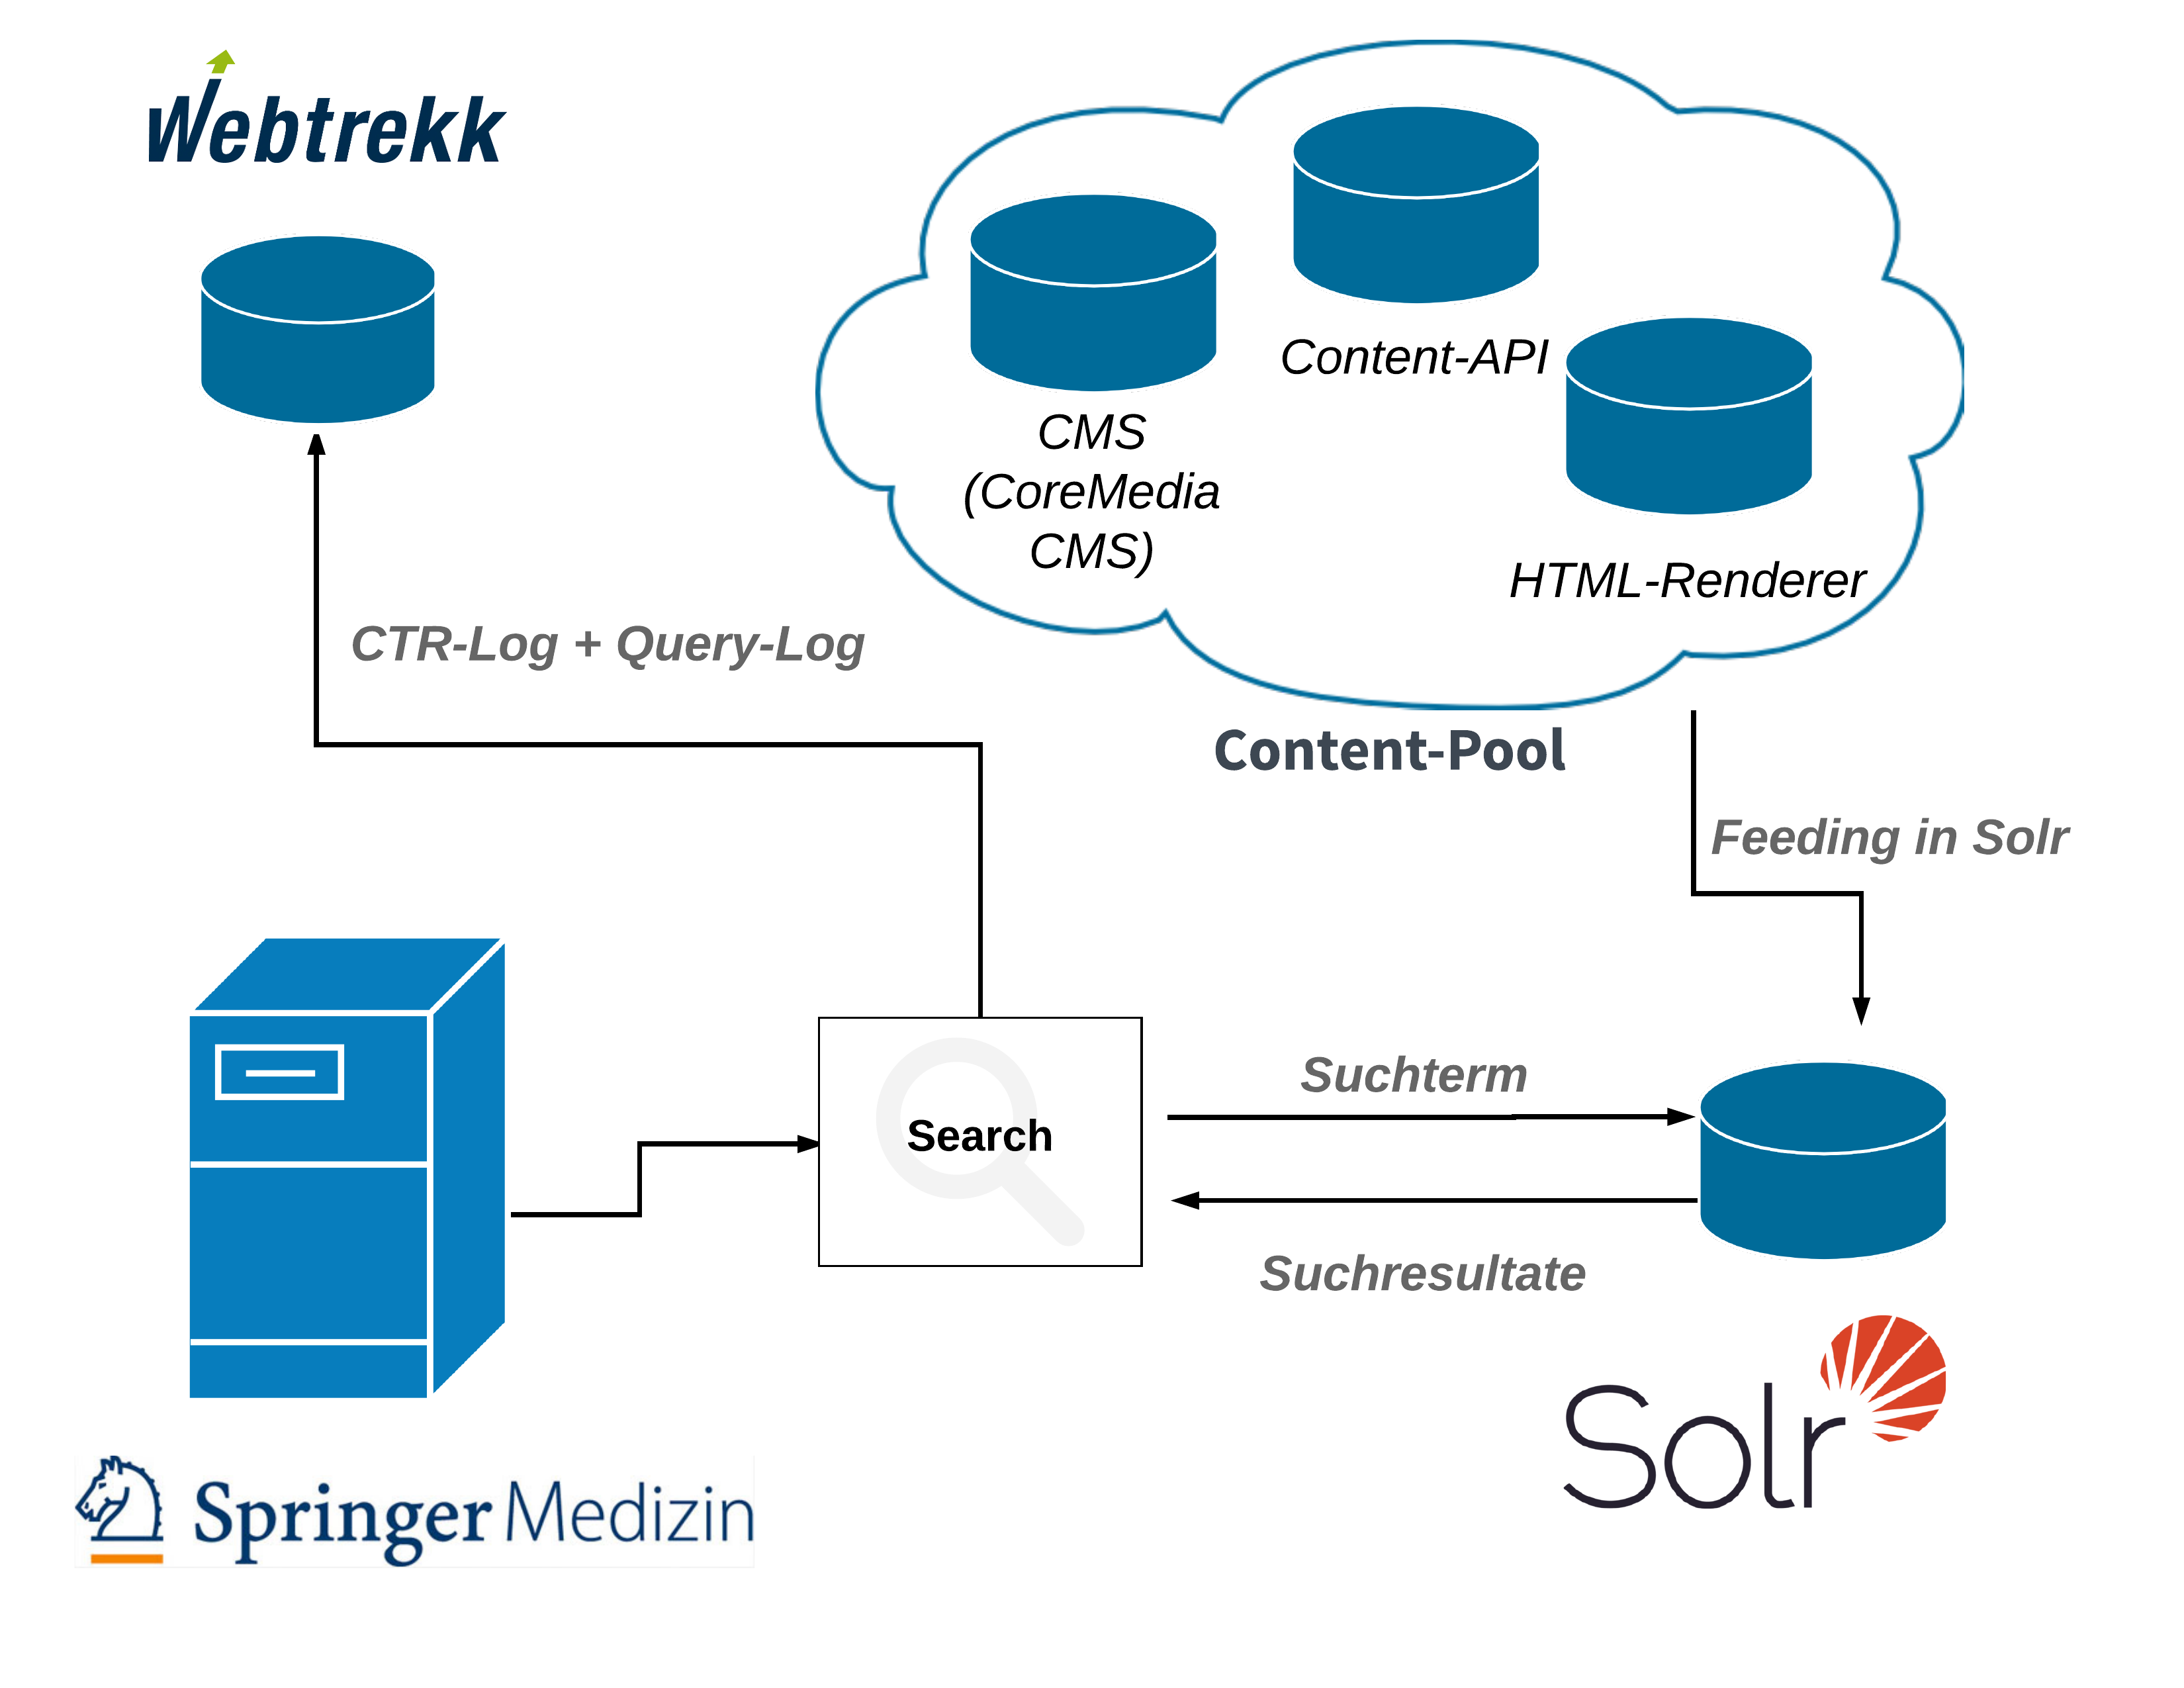
\includegraphics[width=0.7\linewidth]{gfx/AufbauSucheSpringerNature}
\vspace{-2em}
\end{figure}

% Problemstellung: Keine Userrelevanz in der Suche
%------------------------------------------------

\section{Problemstellung: Keine Userrelevanz in der Suche}
\label{sec:Einfuehrung:Problemstellung}

Zu den Stakeholder\footnote{Bezeichnet Springer Nature interne Kunden, die ein Interesse am Ergebnis der White Label Applikation haben}, der in Kapitel \ref{sec:Einfuehrung:AufbauSucheBeiSpringerNature:WhiteLabelApplikationSolr-Suche} angesprochenen White Label Applikation, gehört \textit{Springermedizin}~(siehe \cite{SMED}). Springermedizin betreibt ein Fortbildungs- und Informationsportal für Ärzte.

\subsubsection{Userrelevante Dokumente werden nicht gefunden}
\label{sec:Einfuehrung:Problemstellung:Userrelevanz}

Die User von Springermedizin suchen oft mit einschlägig, fundierten Fachbegriffen nach den neuesten und relevantesten Zeitschriften, Bücher oder Publikationen. Die zeitlich aktuellsten Suchtreffer zu finden ist für Springermedizin kein Problem. Die für den User \textit{relevantesten} jedoch schon.

\subsubsection{Der Springer Nature Stakeholder: Springermedizin setzt auf Webtrekk}
\label{sec:Einfuehrung:Problemstellung:Springermedizin}

Mithilfe von Webanalysten und Webtrekk versucht Springermedizin das Marketing seines Webauftrittes zu verbessern und ist sehr interessiert an neuen Ansätzen um die gesammelten Tracking-Daten besser einzusetzen. In dieser Arbeit wird darum der Fokus auf die Verwendung von Tracking-Daten in der Suche von Springermedizin gesetzt. 
 
\subsubsection{Der fast gläserne User}
\label{sec:Einfuehrung:Problemstellung:Glaeserne-User}

Springermedizin sammelt Tracking-Daten über jegliche Aktivitäten auf deren Applikationen und investiert Zeit und Geld in die Individualisierung\footnote{Mit Individualisierung wird die Speicherung eigener Parameter bezeichnet} der Analysedaten auf Webtrekk. Mittlerweile sind knapp 30 Custom-Parameter\footnote{Individuell erzeugte Parameter für Berichte und Analysen} auf Webtrekk angelegt, um genau die Daten zu tracken, die zur Analyse des Verhaltens der User auf ihrer Applikationen relevant sind. Dadurch entsteht ein fast \glqq gläsernen User\grqq{}. Dieses Wissen könnte zum Vorteil des Users eingesetzt werden indem es in der Suche verwendet wird.

\pagebreak
% Ziel der Arbeit
%------------------------------------------------
\section{Ziel der Arbeit}
\label{sec:Einfuehrung:ZielArbeit}

\subsection{Suchoptimierung durch Click-Through-Daten}
\label{sec:Einfuehrung:ZielArbeit:Suchoptimierung}

In dieser Arbeit werden wir untersuchen ob mithilfe der von Springermedizin gesammelten Click-Through-Daten\footnote{Mit Click-Through-Daten bezeichnen wir alle Tracking-Daten, welche während der Interaktion zwischen User und Suche protokolliert werden} deren Suche verbessert werden kann. Konkret wollen wir dies anhand eines Algorithmus basierend auf dem Klick-Modell\footnote{Als Klick-Modell wird ein Modell zur Berechnung des Userfeedbacks bzw. der Userrelevanz mithilfe von Click-Through-Daten bezeichnet} \textit{Position-Based Modell}~(PBM, siehe \cite{pbm}) untersuchen.

\subsubsection{Annahmen}
\label{sec:Einfuehrung:ZielArbeit:Suchoptimierung:Annahmen}

Wir gehen dabei von zwei Annahmen aus. Zum einen dass relevante Dokumente wichtiger sind, als nicht relevante Dokumente und zum anderen dass ein Suchergebnis dann gut ist, wenn die relevanten Ergebnisse in der verwendeten Hierarchie vor den nicht relevanten Ergebnissen auftauchen. 

\subsubsection{Anwendung auf das Springermedizin-Umfeld}
\label{sec:Einfuehrung:ZielArbeit:Suchoptimierung:AnwendungSpringermedizin-Umfeld}

Wir werden versuchen die CTRs der Suchresultate, mithilfe des oben angesprochenen Algorithmus, zu berechnen und mit diesen ein \textit{Reranking}\footnote{Mit Reranking bezeichnen wie die Umsortierung einer Liste von Suchresultaten} der Suchresultate auf das Springermedizin-Umfeld abzubilden. Die Herausforderung wird hierbei die Adaptierung des Lösungsansatzes auf das Springermedizin-Umfeld sein. Im Idealfall werden die gesammelten Click-Through-Daten die Userrelevanz der einzelnen Dokumente\footnote{Als Dokumente werden die einzelnen Suchresultate bezeichnet} widerspiegeln.

\subsection{Abbildung auf das Springermedizin-Umfeld}
\label{sec:Einfuehrung:ZielArbeit:AbbildungSpringermedizinUmfeld}

\subsubsection{Potential von Userrelevanzen in der Suchoptimierung analysieren}
\label{sec:Einfuehrung:ZielArbeit:Potential}

Die Analyse von User-Tracking-Daten bietet viel Potential bezogen auf Userrelevanzen. Falls anhand des hier umgesetzten Lösungsansatzes Verbesserungen in der Qualität der Suche zu verzeichnen sind, möchte Springermedizin in Zukunft vermehrt User-Tracking-Daten in die Suche einfließen lassen. Diese Arbeit könnte dann als Fundament für weitere Lösungsansätze dienen.

\subsubsection{Bekanntes und wirkungsvolles Information Retrieval Verfahren}
\label{sec:Einfuehrung:ZielArbeit:AbbildungSpringermedizinUmfeld:InformationRetrievalVerfahren}

Suchoptimierung mittels Userrelevanz ist ein bekanntes und nicht triviales, aber relativ wirkungsvolles Information Retrieval Verfahren~(siehe \cite{IWUSBI}). Seit Mitte der 2000er Jahre wird mithilfe dieses Verfahrens versucht Suchmaschinen zu verbessern. Aus dieser Zeit stammen auch die ersten Ansätze, um mithilfe von Click-Through-Daten die Userrelevanz der Suchergebnisse zu berechnen~(siehe \cite{Joachims}).

\subsubsection{Lösungsansatz basierend auf Click-Through-Daten aus Webtrekk}
\label{sec:Einfuehrung:ZielArbeit:AbbildungSpringermedizinUmfeld:Loesungsansatz}

Springermedizin führt ein eigenes Tracking der User durch und verwendet auf Webtrekk selbst definierte Tracking-Parameter. Dadurch hängt die Wahl des in dieser Arbeit zu untersuchenden Lösungsansatzes und dessen Umsetzung stark von den durch Webtrekk gegebenen Analyse-Daten ab.

\subsubsection{Keine Gegenüberstellung mit anderen Lösungsansätzen}
\label{sec:Einfuehrung:ZielArbeit:AbbildungSpringermedizinUmfeld:NichtBehandeln}

Bedingt durch den vorgegebenen Zeitraum für die Erstellung dieser Bachelorarbeit, werden wir den Lösungsansatz so wählen, dass er mit den Gegebenheiten bei Springermedizin sinnvoll und in diesem Zeitrahmen realistisch implementiert werden kann. Wir werden daher in dieser Arbeit keine Gegenüberstellung mit anderen Lösungsansätzen machen. 

% Methodik
%------------------------------------------------

\section{Methodik}
\label{sec:Einfuehrung:Methodik}

Wie in Kapitel \ref{sec:Einfuehrung:ZielArbeit:Suchoptimierung} angesprochen wollen wir das Klick-Verhalten der User in der Suche analysieren um mithilfe der daraus berechenbaren CTRs, die Suchergebnisse zu verbessern. Dieses Klick-Verhalten können wir aus den Click-Through-Daten lesen. 

\subsubsection{Suchterm semantisch aufschlüsseln}
\label{sec:Einfuehrung:Methodik:SuchtermSegmentierung}

Um mit den Click-Through-Daten arbeiten zu können, müssen wir zunächst die relevanten Click-Through-Daten herausfiltern. Dazu müssen wir die Click-Through-Daten dem \textit{Suchterm}\footnote{Als Suchterm wird die Sammlung aller, in der Suchanfrage verwendeten Wörter bezeichnet} der Anfrage zuordnen können. Zu den Click-Through-Daten wird immer der Suchterm gespeichert mit dem dabei gesucht wurde. Das heißt wir können eine Relation zwischen dem Suchterm der Click-Through-Daten und dem Suchterm unserer Anfrage herstellen.
\\
\\
Die Click-Through-Daten müssen aber nicht mit dem vollständigen Suchterm in Relation stehen. Sie können auch nur mit einem Wort, einem Teil des Suchterms oder einem Synonym eines dieser Worte in Relation stehen. Wir müssen darum den Suchterm semantisch aufschlüsseln, um alle relevanten Click-Through-Daten filtern zu können. 

\subsubsection{Aufbereitung Click-Through-Daten}
\label{sec:Einfuehrung:Methodik:Click-Through-Daten}

Können wir alle relevanten Click-Through-Daten zu einer Suchanfrage filtern, müssen wir lernen diese richtig aufzubereiten um die CTR berechnen zu können.  Ein wichtiger Punkt bei der Aufbereitung der Click-Through-Daten ist die Interpretation des Relevanzfeedbacks der einzelnen Click-Through-Daten. Nicht jeder Klick ist gleich relevant zu interpretieren. Die Relevanz eines Klicks hängt davon ab, welche Aktionen der User während dem Suchvorgang \textit{vor} und \textit{nach} dem Klick durchgeführt hat. Wir müssen darum zuerst analysieren, welche Informationen wir zu den Click-Through-Daten aus Webtrekk lesen können.  Reichen diese Informationen für detailliertere Interpretationen nicht aus, müssen wir alle Click-Through-Daten als gleich relevant lesen.

\subsubsection{Result-Reranking mittels PBM basierten Algorithmus}
\label{sec:Einfuehrung:Methodik:Result-RerankingPBM}

Sobald wir wissen wie man die Click-Through-Daten aufbereitet, können wir diese zur Berechnung der CTR eines Dokumentes, und somit dessen Userrelevanz, einsetzen. Für die Verwendung dieser Userrelevanz müssen wir festlegen, wann und in welcher Art wir sie einsetzen. Wie bereits in Kapitel \ref{sec:Einfuehrung:ZielArbeit:Suchoptimierung:AnwendungSpringermedizin-Umfeld} erwähnt, werden wir uns in dieser Arbeit auf die \textit{Aufbereitung} der Suchresultate aus der Solr konzentrieren und dort einen \textit{Reranking-Algorithmus} einbauen. 
\\
\\
Der Reranking-Algorithmus basiert auf dem \textit{Klick-Modell PBM}. Ein Klick-Modell verwendet die Click-Through-Daten, um daraus die CTR eines Dokumentes zu berechnen. Die Wahl des Klick-Modells hängt darum stark von den Click-Through-Daten und den darin enthaltenen Informationen ab. Das PBM setzt sich aus zwei Wahrscheinlichkeiten zusammen. Die Wahrscheinlichkeit für einen Klick auf die Position im Suchresultat und die Wahrscheinlichkeit für einen Klick auf das Dokument. In dieser Arbeit werden wir veranschaulichen, warum wir den Ansatz des PBMs~(siehe \cite{pbm}) gewählt haben und wie wir den Algorithmus umgesetzt haben.

\subsubsection{Vergessen der alten Daten}
\label{sec:Einfuehrung:Vergessen}

Das PBM berechnet Wahrscheinlichkeiten, um die CTR eines Dokumentes zu einer Suchanfrage festzustellen. Dem Algorithmus muss dazu das notwendige Wissen entweder zur Verfügung gestellt oder antrainiert werden. Wird dem Algorithmus das Wissen antrainiert, benötigt der Algorithmus eine Möglichkeit neues Wissen zu Lernen und Altes zu vergessen. 
\\
\\
Mit Webtrekk haben wir eine Wissensbasis, die durch die Springermedizin-Applikation automatisch um neue Click-Through-Daten ergänzt wird. Das heißt wir müssen uns nicht um eine Möglichkeit zum Lernen neuer Daten kümmern. Wir müssen uns aber überlegen, wie wir altes Wissen vergessen und wie wir dem User neues Wissen präsentieren, damit dieser sich durch die CTR-Berechnung nicht auf alten Dokumenten festfährt.

% Gliederung und Aufbau
%------------------------------------------------

\section{Gliederung und Aufbau}
\label{sec:Einfuehrung:GliederungAufbau}

\subsubsection{Der Lösungsansatz und deren Grundlagen}
\label{sec:Einfuehrung:GliederungAufbau:Loesungsansatz}

In diesem Kapitel wurde der zu untersuchende Lösungsansatz vorgestellt. Wir haben Problemstellungen und deren Teilprobleme identifiziert. Dabei sind wir auf die Hintergründe dieser Arbeit und die Vorgehensweise eingegangen. Im zweiten Kapitel~(Grundlagen) folgt die Theorie des beschriebenen Lösungsansatzes. Hier werden wir uns auf die fachlichen Grundlagen konzentrieren, Problemstellungen analysieren und Lösungsansätze vorstellen.

\subsubsection{Umsetzung des Lösungsansatzes}
\label{sec:Einfuehrung:GliederungAufbau:Umsetzung}

In Kapitel \ref{sec:Reranking}~(Reranking mittels CTR) werden wir die in Kapitel \ref{sec:Einfuehrung:Methodik} angesprochene Methodik verfeinern und auf Basis der Grundlagen aus Kapitel \ref{sec:Grundlagen:Grundbegriffe}, über die detaillierte Vorgehensweise bei der Umsetzung diskutieren. Die Umsetzung selbst folgt dann in Kapitel \ref{sec:Implementierung}~(Implementierung).

\subsubsection{Erkenntnisse verarbeiten}
\label{sec:Einfuehrung:GliederungAufbau:Erkenntnisse}

Um zu prüfen ob der umgesetzte Lösungsansatz die erhofften Verbesserungen erzielt, werden wir diesen in Kapitel \ref{sec:Evaluation}~(Evaluation und Auswertung) in einer Evaluation mit der bisherigen Springermedizin-Suche vergleichen. Aufgrund der resultierenden Erkenntnisse, werden wir in Kapitel \ref{sec:ZusammenfassungAusblick}~(Zusammenfassung und Ausblick) ein Fazit ziehen können und einen Ausblick auf mögliche, zukünftige Arbeiten geben. 			% INCLUDE: Einführung
% !TEX root = ../thesis-example.tex
%
%************************************************
% Grundlagen
%************************************************
\chapter{Grundlagen}
\label{sec:Grundlagen}

% Grundbegriffe
%************************************************

\section{Grundbegriffe}
\label{sec:Grundlagen:Grundbegriffe}

In diesem Kapitel werden wir die fachlichen Grundlagen zu unserem in Kapitel \ref{sec:Einfuehrung:Methodik} vorgestellten Lösungsansatz aufarbeiten. Wichtig hierfür ist das Verständnis für die Problemstellungen in der Interaktion zwischen den Nutzern der Suche und der Suche selbst und warum unser verfolgter Lösungsansatz schief gehen kann. Dazu gehört die Auseinandersetzung mit dem Klick-Verhalten der User auf der Suche von Springermedizin. Mit der Click-Trough-Rate wollen wir eine Userrelevanz bestimmen. Dazu müssen wir die Click-Trough-Daten als Relevanz-Feedback deuten können. Wie wir die Click-Trough-Rates berechnen, lernen wir in den Grundlagen zu unserem Reranking-Algorithmus. Diese Grundlagen sind notwendig für die Umsetzung des Lösungsansatzes in den nachfolgenden Kapiteln \ref{sec:Reranking} und \ref{sec:Implementierung}. In diesem Kapitel und dem darauf folgenden, werden Formeln mit selbst definierten Symbolen eingeführt. Folgend eine Legende zu den wichtigsten Symbolen:

\begin{table}[H]
\centering
\vspace{-.5em}
\caption[Legende der wichtigsten Formel-Symbolen für diese Arbeit]{Legende der wichtigsten Formel-Symbolen für diese Arbeit}
\label{tab:LegendeSymboleFormeln}
\vspace{-.5em}
\footnotesize
\renewcommand*{\arraystretch}{1.2}
\begin{tabular}{clcl} \hline
\textbf{Symbol} & \textbf{Bedeutung} & \textbf{Symbol} & \textbf{Bedeutung} \\ \hline
$u$	& ein Dokument im Suchergebnis & $C$	& das Dokument wird vom User \\ &&& im Suchergebnis angeklickt \\ 
$q$	& ein Suchterm & $E_{u}$	& das Dokument wird aufgrund seiner Position \\ &&& im Suchergebnis angeschaut \\
$r$	& die Position des Dokumentes im Suchergebnis &  $A_{u}$	& das Dokument wird aufgrund seines Suchsnippets \\ &&& im Suchergebnis angeschaut \\ 
$c$	& ein Klick auf ein Dokument im Suchergebnis & $X_{u}$	& ein Zufallswert der einem Dokument \\ &&& des Suchergebnisses zugewiesen wird \\
$s$ 	& eine Suchanfrage & $r_{X_{u}}$	& $r$ in der nach Zufallsfaktor \\ &&& sortierten Liste der Suchergebnisse \\ 
$S$	& eine Set von Suchanfragen & $r_{P(C_{u})}$ 	& $r$ in der nach Klick-Wahrscheinlichkeit \\ &&& sortierten Liste der Suchergebnisse \\
$P$	& die Wahrscheinlichkeit dass ein Fall eintritt &  $R_{u}$	& durch den Reranking-Algorithmus berechneter \\ &&& Relevanz-Wert des Dokumentes $u$ \\
\hline
\end{tabular}
\vspace{-2em}
\end{table}

% Semantik von User-Interaktionen
%------------------------------------------------

\subsection{Semantik von User-Interaktionen}
\label{sec:Grundlagen:Grundbegriffe:SemantikUserInteraktionen}

\subsubsection{Problemstellungen der Click-Trough-Daten: Was analysieren wir?}
\label{sec:Grundlagen:Grundbegriffe:SemantikUserInteraktionen:ProblemstellungenClick-Trough-Daten}

\paragraph{Einzelne Wörter oder Teile des Suchterms können in weiteren Suchanfragen vorkommen}
Ein Suchterm kann aus einem oder mehreren Wörtern bestehen. Jeder User formuliert eine Suchanfrage anders. Sei es die Wortwahl, die Zeitform oder die Verwendung von Bindewörtern. Daraus lässt sich vermuten, dass einzelne Wörter oder Teile des Suchterms in weiteren Suchanfragen vorkommen können. Folglich muss der Suchterm semantisch aufgeschlüsselt werden, um Relationen zwischen Click-Trough-Daten und der Suchanfrage herstellen zu können. Nur so können wir alle relevanten Click-Trough-Daten filtern.

\paragraph{Suchanfragen mit Synonymen und verwandten Begriffen beachten}
Nehmen wir als Beispiel die Suchanfrage \glqq chronische Dyspnoe\grqq{}. Würden wir stattdessen den sinnverwandten Suchterm \glqq konstante Atemnot\grqq{} verwenden, würden wir für beide Fälle ähnliche Suchresultate erwarten. Folglich würden wir auch ähnliche Click-Trough-Daten vermuten. Wir sollten daher die Synonyme und verwandte Begriffe zu unserem Suchterm ebenfalls beachten und deren Click-Trough-Daten, in den Reranking-Algorithmus einfließen lassen. Dazu benötigen wir eine Wissensbasis, welche die Synonyme und verwandte Begriffe zu unserem Suchterm gespeichert hat. Eine solche Basis bieten Wörterbücher und Thesauri\footnote{Thesauri sind strukturierte Verzeichnisse von Begriffen, die allesamt in irgendeiner Beziehung zueinander stehen bezeichnet}. Beim Content von Springermedizin handelt es sich um medizinische Inhalte in deutscher Sprache. Es macht daher Sinn dies in der Wahl der richtigen Wissensbasis zu berücksichtigen.

\subsubsection{Problemstellungen des Lösungsansatzes: Warum kann es schief gehen?}
\label{sec:Grundlagen:Grundbegriffe:SemantikUserInteraktionen:ProblemstellungenLoesungsansatz} 

Die folgenden Faktoren leiten sich aus dem verfolgten Lösungsansatz des Reranking-Algorithmus ab, bzw. werden in diesem nicht beachtet. Wir müssen davon ausgehen dass diese das Untersuchungsergebnis des Lösungsansatzes negativ beeinflussen könnten.

\paragraph{Die Relation des Suchterms zu den Click-Trough-Daten wird nicht gewichtet}
Die Click-Trough-Daten sind dann relevant, wenn mindestens ein Wort des aufgeschlüsselten Suchterms in Relation zu diesen Daten steht. Dadurch können falsche Relationen entstehen und nicht relevante Click-Trough-Daten die Klick-Wahrscheinlichkeiten der Dokumente im Reranking-Algorithmus negativ beeinflussen.

\paragraph{Intentionen und die Mehrdeutigkeit von Suchbegriffen werden nicht beachtet}
Die genaue semantische Analyse eines Suchterms beinhaltet unter anderem die Erkennung von Begriffen und deren Mehrdeutigkeiten. Suchte jemand z.B. nach dem Begriff \glqq Brücke\grqq{}, hat dieser im medizinischen Kontext mehrere Bedeutungen. Es könnte ein \glqq ein Teil des zentralen Nervensystems\grqq{} gemeint sein oder eine \glqq Form des Zahnersatzes\grqq{}. Wie bereits im vorherigen Kapitel \ref{sec:Grundlagen:SemantikUserInteraktionen:ProblemstellungenClick-Trough-Daten} erwähnt, können wir mithilfe eines Thesaurus die verschiedenen Bedeutungen erkennen. Unser Reranking-Algorithmus ignoriert diese Mehrdeutigkeit jedoch. Er würde in diesem Fall alle Click-Trough-Daten zu beiden Begriffsbedeutungen suchen. Hier können wir zufallsbedingt drei Ausgangslagen haben. Die Click-Trough-Daten entsprechen der Suchintention (1) - das wäre der zufallsbedingte Optimalfall. Das Suchresultat würde von der Mehrfachbedeutung nicht beeinflusst werden. Tritt das Gegenteil ein (2) - Das Suchresultat wird in diesem Fall durch eine falsche Relevanz negativ beeinflusst. Keine Click-Trough-Daten vorhanden (3) - Die Volltextsuche und die Klick-Wahrscheinlichkeit der Position im Suchresultat definieren das Suchergebnis. In diesem Fall kann die Wertigkeit des Algorithmus nicht vorhergesehen werden.

\paragraph{Keine Aktualität in der Suche}
Der von uns verfolgte Reranking-Algorithmus nimmt keine Rücksicht auf die \glqq Aktualität\grqq{} eines Beitrages sondern nur auf die Klick-Wahrscheinlichkeit und könnte dadurch aktuellere Dokumente trotz Relevanz, schlecht positionieren im Suchresultat.  Die Klick-Wahrscheinlichkeit kann durch zwei Faktoren beeinflusst werden. Hohe Relevanz in der Solr-Suche (1) - wird in der Volltextsuche die Aktualität des Dokumentes in die Berechnung der Relevanz einbezogen, werden aktuelle Beiträge im Suchergebnis der Solr weit vorne eingestuft. Wie wir aus Abb. \ref{fig:Grundlage:AnalyseKlicksPositionen} erkennen können, haben niedrige Positionen eine höhere Klick-Wahrscheinlichkeit. Das könnte die Berechnung des Reranking-Algorithmus positiv beeinflussen. Reranking-Algorithmus um Zufallsfaktor erweitern (2) - mithilfe eines Zufallsfaktor ist die Reihenfolge der Suchresultate weniger vom Algorithmus abhängig und die Wahrscheinlichkeit, aktuelle Dokumente ohne Click-Trough-Daten weit vorne im Suchergebnis zu finden wird erhöht.

\paragraph{Interessante Dokumente werden nie gesehen}
Wie bereits oben erwähnt, beachtet der Reranking-Algorithmus Dokumente ohne Click-Trough-Daten nur, wenn die Position im Suchresultat eine Klick-Wahrscheinlichkeit aufweist. Dadurch kann es sein, dass interessante Dokumente nie gesehen werden. Dem entgegenwirken können wir ebenfalls mit dem oben erwähnten Zufallsfaktor. Dadurch wird die Klick-Wahrscheinlichkeit für interessante Dokumente zufallsbedingt erhöht.

\subsubsection{Nicht beeinflussbare Faktoren: Fehlerhafter Content verfälscht die Suchergebnisse}
\label{sec:Grundlagen:Grundbegriffe:SemantikUserInteraktionen:FehlerhafterContent}

Die folgenden Faktoren beeinflussen das Suchergebnis negativ, sind aber vom Content so vorgegeben. Der von uns verfolgte Lösungsansatz des Reranking-Algorithmus kann diese nicht beeinflussen. Wir beachten diese Faktoren in unserer Arbeit darum nicht.

\paragraph{Mehrfachverwertung des Contents}
Auf der Springermedizin Suche wird teilweise im Suchergebnis auf denselben Artikel mehrfach  verwiesen. Das liegt an der bei Springermedizin praktizierten Mehrfachverwertung des Contents. Es gibt \textit{Journal-Artikel}, das sind aus Journalen, Zeitschriften oder Magazinen stammende Artikel, die auf Springermedizin direkt online\footnote{Der Begriff \glqq online\grqq{} wird hier als Verweis auf die Springermedizin.de-Webseite verwendet} gelesen werden können. Bei Neuerscheinung des Artikels, werden dazu oft redaktionelle Artikel publiziert, welche auf den Journal-Artikel verweisen sollen. Diese können im CMS (siehe Abb. \ref{fig:SucheSpringerNature}) von der Suche exkludiert werden. Werden diese nicht exkludiert, können beide Artikel im Suchergebnis erscheinen.

\paragraph{Ausspielung von Teaser}
Springermedizin verwendet Teaser\footnote{Als Teaser wird ein kurzer Texte bezeichnet, der das Interesse für den nachfolgenden Beitrag wecken soll} auf der Startseite und auf Übersichtsseiten zu Rubriken als Einstieg in den nachfolgenden ausführlichen Beitrag. Diese werden auch in der Suche ausgespielt. Teaser sagen nichts über die Wertigkeit des Beitrages aus. Man weiß nicht, auf welche Art von Beitrag (z.B wissenschaftliche Publikation oder ein Artikel aus ein Journal) verwiesen wird und von welchem Autor der Beitrag stammt. Sie können darum nicht nach Relevanz eingestuft werden und sollten darum nicht im Suchergebnis erscheinen.

\paragraph{Fehlerhafte Importe der Daten}
Viele Beiträge sind falschen Rubriken zugeordnet. Beispielsweise werden Beiträge fälschlicherweise als wissenschaftliche Publikationen publiziert, obwohl sie aus einem Journal oder einer Fachzeitschrift stammen. Diese Fehler sind auf fehlerhafte Importe der Daten zurückzuführen und verfälschen die Wertigkeit des Suchergebnisses.

\paragraph{Schlechte Suchsnippets beeinflussen die Klick-Wahrscheinlichkeit eines Dokumentes negativ}
Das Position-Based Modell berechnet die Klick-Wahrscheinlichkeit, also die \textit{Attraktivität} eines Dokumentes auf Basis dessen Klick-Häufigkeit zum Suchterm und dessen Position im Suchresultat. Das heißt der User analysiert das Suchresultat und sobald er auf den Link zu einem Dokument klickt, fließt dieser Klick in die Berechnung ein. Folglich bestimmt nicht der Inhalt des Dokumentes über dessen Attraktivität, sondern dessen Suchsnippet\footnote{Unter einem Suchsnippet wird eine Zusammenfassung des Inhalts des verlinkten Dokumentes als kurzen Teasertext verstanden}. Wirkt dieses wenig relevant, kann dadurch die Klick-Wahrscheinlichtkeit negativ beeinflusst werden.

\subsubsection{Analyse der Click-Trough-Daten: Wenige Dokumente erhalten viele Klicks}
\label{sec:Grundlagen:Grundbegriffe:SemantikUserInteraktionen:DocumentAttraction}


Um das Klick-Verhalten der User auf der Springermedizin-Suche zu verstehen, ist es wichtig anhand oft gesuchter Suchphrasen dieses Verhalten zu analysieren. Dazu wurde eine Analyse über einen Zeitraum von 30 Tagen erstellt und die zehn am häufigsten gesuchten Suchphrasen verwendet. Die Analyse vergleicht für jede Suchphrase die 20 Dokumente mit den meisten Klicks. Die Dokumente wurden hierbei nicht nach Position im Suchergebnis sondern nach Klick-Häufigkeit selektiert. Jeder Graph der folgenden Abbildung \ref{fig:Grundlagen:AnalyseKlicksTop10Suchergebnisse} stellt eine Suchphrase dar. Wie wir sehen, zeigen die meisten Graphen ein exponentiell stark abnehmendes Verhalten der Klick-Häufigkeiten. Dieses exponentielle Verhalten zeigt, dass einzelne Dokumente häufig und viele Dokumente selten bis nie angeklickt werden. Dieser Effekt kann wie in vielen natürlichen Phänomenen mit exponentiellem Verhalten, durch das Potenzgesetz (Power Law, siehe \cite{PowerLaw}) beschrieben werden. 

\begin{figure}[H]
\centering 
\vspace{-1em}
\caption[Analyse der 20 am häufigsten angeklickten Dokumente  der zehn meistgesuchten Suchphrasen. \textit{Zeitraum der Analyse: 19.08.16 - 19.09.16}]{Analyse der 20 am häufigsten angeklickten Dokumente  der zehn meistgesuchten Suchphrasen. \\ \textit{Zeitraum der Analyse: 19.08.16 - 19.09.16}}
\label{fig:Grundlagen:AnalyseKlicksTop10Suchergebnisse}
 
\pgfplotstableread[col sep=semicolon]{content/diagrams/clicks_top10_searchphrases_result.csv}\topSearchphrases
  
\begin{tikzpicture}
\begin{axis}[
	width=14cm,
	height=5cm,
	scale only axis,
	xmajorgrids,
	xminorgrids,
    ylabel=\textbf{Anzahl der Klicks}, 
	xlabel=\textbf{Dokumente sortiert nach Anzahl der Klicks},
    xtick=data,
    ymin=0,
    xmin=1,
    xmax=20,
    legend pos=north east,
    legend style={font=\tiny}
]
\addplot table [
    x=S1,
    x=Position
] {\topSearchphrases};
\addplot table [
    y=S2,
    x=Position
] {\topSearchphrases};
\addplot table [
     y=S3,
    x=Position
] {\topSearchphrases};
\addplot table [
     y=S4,
    x=Position
] {\topSearchphrases};
\addplot table [
     y=S5,
    x=Position
] {\topSearchphrases};
\addplot table [
     y=S6,
    x=Position
] {\topSearchphrases};
\addplot table [
     y=S7,
    x=Position
] {\topSearchphrases};
\addplot table [
     y=S8,
    x=Position
] {\topSearchphrases};
\addplot table [
     y=S9,
    x=Position
] {\topSearchphrases};
\addplot table [
     y=S10,
    x=Position
] {\topSearchphrases};
\legend{borreliose ($1015$ Suchergebnisse), copd ($17337$ Suchergebnisse), dgrm-jahrestagung $2016$ ($18$ Suchergebnisse), diabetes ($148755$ Suchergebnisse), dyspnoe ($10601$ Suchergebnisse), forensische traumatologie ($150$ Suchergebnisse), gicht ($1188$ Suchergebnisse), hypertonie ($12765$ Suchergebnisse), mmw ($12666$ Suchergebnisse), vorhofflimmern ($4981$ Suchergebnisse)}
\end{axis}
\end{tikzpicture}

\vspace{-2em}
\end{figure}

Betrachten wir die Graphen, können wir vor allem für die ersten fünf analysierten Dokumente verglichen mit den restlichen analysierten Dokumenten, hohe Klick-Häufigkeiten feststellen. Daraus lässt sich die Vermutung ableiten, dass einzelne Dokumente eine sehr hohe Relevanz für die entsprechende Suchanfrage aufweisen und nur wenige Dokumente auf die User als relevant wirken. Ein weitere Vermutung ist, dass der zu durchsuchende Content wenig relevante Dokumente hat. Die Suchphrasen lassen auf sehr diverse Suchintentionen deuten. Es handelt sich hierbei unter anderem um Krankheiten, Zeitschriften und Behandlungen mit mehreren tausend Suchergebnissen. Die Wahrscheinlichkeit, dass wenig relevanter Content für die meisten der analysierten Suchphrasen zutrifft, sollte aufgrund der hohen Anzahl an gefundenen Suchergebnissen zu diesen Suchphrasen, relativ gering sein. Wir müssen darum eher davon ausgehen, dass sich die User auf einzelne im Suchresultat weit oben stehende Dokumente festfahren. Das könnte an schlechten Suchergebnissen und somit an einer schlechten Suchqualität liegen. Um jedoch ein genaueres Bild über das Verhalten erstellen zu können müssen wir einen Vergleich mit der nachfolgenden Analyse in Abbildung \ref{fig:Grundlage:AnalyseKlicksPositionen} ziehen.

\subsubsection{Analyse der angeklickten Positionen: Niedrige Positionen werden häufiger angeklickt}
\label{sec:Grundlagen:Grundbegriffe:SemantikUserInteraktionen:RankExamination}


In der unten folgenden Analyse sehen wir das positionsbezogene Klick-Verhalten der User auf der Springermedizin-Suche. Dazu wurden über den Zeitraum von einem Monat, die letzten 1000 Suchanfragen ausgewertet. Dargestellt sehen wir die Häufigkeitsverteilung der Klicks als Graph. Wir beschränken uns hierbei auf die ersten 20 Positionen der Suchresultate. Wie wir sehen, nimmt die Anzahl der Klicks mit zunehmender Position exponentiell ab. Dieser Effekt kann ebenfalls, wie in Abb. \ref{fig:Grundlagen:AnalyseKlicksTop10Suchergebnisse}, durch das Potenzgesetz (Power Law, siehe \cite{PowerLaw}) beschrieben werden. 

\begin{figure}[H]
\centering 
\vspace{-1em}
\caption[Analyse der Klicks auf die ersten 20 Positionen der Suchergebnisse aller Suchanfragen. \textit{Zeitraum der Analyse: 19.08.16 - 19.09.16}]{Analyse der Klicks auf die ersten 20 Positionen der Suchergebnisse aller Suchanfragen. \\ \textit{Zeitraum der Analyse: 19.08.16 - 19.09.16}}
\label{fig:Grundlage:AnalyseKlicksPositionen}

\footnotesize
\pgfplotstableread[col sep=semicolon]{content/diagrams/clicks_top1000_ranks_result.csv}\topRanks
  
\begin{tikzpicture}
\begin{axis}[
	width=14cm,
	height=3cm,
	scale only axis,
	xmajorgrids,
	xminorgrids,
    ylabel=\textbf{Anzahl der Klicks}, 
	xlabel=\textbf{Position im Suchergebnis},
	nodes near coords, 
	 every node near coord/.append style={xshift=+10pt,yshift=-1pt},
    xtick=data,
    ymin=0,
    xmin=1,
    xmax=20,
    legend style={font=\tiny}
]
\addplot table [
    x=Position,
    y=Klicks
] {\topRanks};
\legend{Anzahl Klicks}
\end{axis}
\end{tikzpicture}

\vspace{-2em}
\end{figure}

Betrachten wir den Graphen, sehen wir, dass besonders die erste Position, auffällig oft angeklickt wird. Daraus könnten wir die Vermutungen ableiten, dass die Suche eine sehr gute Qualität besitzt, weil die zu oberst angezeigten Dokumente, sehr relevant sind und die meisten User der Suchmaschine vertrauen. Wie wir aus den Analysen von \cite{Joachims} lesen können, müssen wir davon ausgehen, dass die Häufigkeit des Klicks auf die ersten Positionen des Suchresultates eher dem Vertrauen der User der Suchmaschine, als der Qualität der Suche geschuldet ist. Vergleichen wir die Analyse aus Abb. \ref{fig:Grundlagen:AnalyseKlicksTop10Suchergebnisse} mit dieser Analyse, sehen wir ein sehr ähnliches Muster in der Häufigkeitsverteilung der Klicks. Wir können anhand der Klick-Zahlen ebenfalls vermuten, dass die am häufigsten angeklickten Dokumente, sich dabei auf den ersten Positionen des Suchergebnisses befunden haben.

% Userrelevanz mittels Click-Trough-Rate (CTR)
%------------------------------------------------

\subsection{Userrelevanz mittels Click-Trough-Rate (CTR)}
\label{sec:Grundlagen:Grundbegriffe:Click-Trough-Daten}

Um mit Click-Trough-Daten arbeiten zu können, müssen wir zuerst verstehen, was Click-Trough-Daten sind und wie sie entstehen. 

\subsubsection{Was sind Click-Trough-Daten und wie entstehen diese?}
\label{sec:Grundlagen:Grundbegriffe:Click-Trough-Daten:WasSindClick-Trough-Daten}

Click-Trough-Daten sind Tracking-Daten. Tracking-Daten entstehen durch die Interaktion zwischen dem User der Applikation und der Applikation selbst. Sie verfolgen das Verhalten der User auf der Applikation und speichern diese in einer Datenbank, in unserem Fall in Webtrekk ab. Die für uns interessanten Tracking-Daten entstehen, wenn der User auf der Suche von Springermedizin ein Anfrage stellt und darauf folgend, ein Element aus dem Suchresultat anklickt.

\subsubsection{Wie werden die Click-Trough-Daten in Webtrekk gespeichert?}
\label{sec:Grundlagen:Grundbegriffe:Click-Trough-Daten:SpeichernClick-Trough-Daten}

Die Speicherung der Daten auf Webtrekk übernimmt die Springermedizin-Applikation. Führt ein User eine Suche durch und klickt dabei ein Resultat an, sendet die Springermedizin-Applikation die Tracking-Informationen an Webtrekk. Die Tracking-Daten für diese Aktion, setzen sich zusammen aus der Suchanfrage, dem Zeitpunkt der Suche, den Userdaten, der angeklickten Position im Suchresultat und den Dokumentinformationen zum angeklickten Dokument.

\subsubsection{Wie können wir Click-Trough-Daten aus Webtrekk lesen?}
\label{sec:Grundlagen:Grundbegriffe:Click-Trough-Daten:LesenClick-Trough-Daten}

Webtrekk ist ein Analysetool. Das heißt für uns, wir können nicht direkt auf die Datenbank mit den Tracking-Daten zugreifen. Um die Tracking-Daten lesen zu können, müssen wir eine Analyse auf Webtrekk ausführen. Mithilfe dieser Analyse können wir uns die Click-Trough-Daten so zusammenstellen lassen, wie wir sie für die Berechnung der Click-Trough-Rate benötigen.

\paragraph{Klick-Häufigkeiten zu Suchterm selektieren und mittels Filtern einschränken} 
Die Click-Trough-Daten bestehen aus einzelnen \textit{Klick-Häufigkeiten}. Eine Klick-Häufigkeit beschreibt die Anzahl der Klicks, die zu einer bestimmten Suchanfrage auf ein bestimmtes Dokument gemacht wurden und auf welcher Position im Suchresultat sich dieses Dokument dabei befunden hat. Die Webtrekk-Analysen geben uns eine Sammlung von Klick-Häufigkeiten zurück. Wir können bei diesen Analysen die Klick-Häufigkeiten nach Suchbegriffen filtern und den Zeitraum mitgeben, in welchen die Suchanfragen durchgeführt wurden. Des weiteren gibt es die Möglichkeit, weitere Filter wie die Anzahl zurückzugebender Klick-Häufigkeiten oder auch den \glqq Login-Status\footnote{Mit Login-Status wird zwischen einem zum Zeitpunkt der Suche auf der Springermedizin-Applikation angemeldeten und nicht angemeldeten User unterschieden} des Users\grqq{} zu setzen. 

\subsubsection{Wie sehen die Click-Trough-Daten aus?}
\label{sec:Grundlagen:Grundbegriffe:Click-Trough-Daten:AussehenClick-Trough-Daten}

Eine Beispiel für eine Klick-Häufigkeit wie er von einer Webtrekk-Analyse ausgespielt wird, sieht wie folgt aus:

\begin{table}[H]
\centering
\vspace{-.75em}
\caption[Beispiel Click-Trough-Daten]{Beispiel Click-Trough-Daten}
\vspace{-.5em}
\label{tab:BeispielCTDaten}
\begin{tabular}{|p{0.8\textwidth}|p{0.15\textwidth}|}\hline
	\textbf{Click-Trough-Daten} & \textbf{Klick-Häufigkeit} \\ \hline
	searchresult-1.Course.chronische Dyspnoe bei Erwachsenen.10621768.chronische Dyspnoe & 5 \\ \hline
 \end{tabular}
\vspace{-2em}
\end{table}

Hier die Aufschlüsselung der Click-Trough-Daten:

\begin{table}[H]
\centering
\vspace{-.75em}
\caption[Beispielhafte Aufschlüsselung der Click-Trough-Daten]{Beispielhafte Aufschlüsselung der Click-Trough-Daten}
\label{tab:AufschluesselungCTDaten}
\vspace{-.5em}
\begin{tabular}{|p{0.15\textwidth}|p{0.15\textwidth}|p{0.27\textwidth}|p{0.1\textwidth}|p{0.2\textwidth}|}\hline
	\textbf{Position} & \textbf{Dokumenttyp} & \textbf{Titel} & \textbf{ID} & \textbf{Suchterm} \\ \hline
	searchresult-1 & Course & chronische Dyspnoe bei Erwachsenen & 10621768 & chronische Dyspnoe \\ \hline
\end{tabular}
\vspace{-2em}
\end{table}

Die Click-Trough-Daten lassen sich wie folgt lesen. In diesem Beispiel haben die User mit der Suchanfrage \glqq chronische Dyspnoe\footnote{Als Dyspnoe wird eine unangenehm erschwerte Atemtätigkeit bezeichnet}\grqq{} gesucht. Dabei haben sie das Dokument mit der ID 10621768 angeklickt. Dieses hat sich dabei auf der Position eins der Suchresultate befunden. Es wurde insgesamt fünfmal angeklickt in der gesuchten Periode. 

\subsubsection{Aus Merkmalen und Eigenschaften des Userverhaltens ein implizites Feedback bilden}
\label{sec:Grundlagen:Grundbegriffe:Click-Trough-Daten:UserverhaltensFeedback}

Mit dem Tracking der User auf einer Suchmaschine verfolgen wir die Idee, ein implizites Feedback aus deren Verhalten interpretieren zu können. Das machen wir, indem wir Merkmale und Eigenschaften des Verhaltens lesen und daraus ein Feature-Set\footnote{Mit Feature-Set bezeichnen wir eine Sammlung von Merkmalen und Eigenschaften zum Userverhalten auf der Suchmaschine}, wie in \cite{IWUSBI} beschrieben erzeugen. Dieses Feature-Set setzt sich zusammen aus den Informationen des \textit{Klick-Verhaltens} der User (Click-Trough Features) und deren \textit{Browsing-Verhalten}\footnote{Mit Browsing wird hier das Verhalten des Users bei der Navigation durch die Suche beschrieben} (Browsing Features) während einer Suchanfrage und den \textit{semantischen Relationen} zwischen der Suchanfrage und den dazu ausgespielten Suchresultaten (Query-Text Features). Mithilfe des Feature-Set lassen sich dann  Schlussfolgerungen zum Relevanz-Feedback ziehen. Auf diesem Feature-Set werden wir bei der Auswertungen unserer Click-Trough-Daten aufbauen, um damit unsere Click-Trough-Rates zu berechnen.

% Result-Reranking mittels PBM Algorithmus
%------------------------------------------------

\subsection{Result-Reranking mittels PBM basierten Algorithmus}
\label{sec:Grundlagen:Grundbegriffe:Result-RerankingPBM}

\subsubsection{Alternative Ansätze um Click-Trough-Daten in den Suchprozess einzubinden}
\label{sec:Grundlagen:Grundbegriffe:Result-RerankingPBM:AlternativenSucheEinbinden}

\paragraph{Kurzanalyse der möglichen Ansätze um Click-Trough-Daten in Suchprozess einzubinden} 
Wir untersuchen in dieser Arbeit die Verwendung der Click-Trough-Daten in der Aufbereitung der Suchresultate der Springermedizin-Applikation. Es gibt aber auch andere mögliche Eingriffspunkte während des Suchprozesses, um die Click-Trough-Daten zu verwenden. Eine Alternative wäre die Verwendung der Click-Trough-Rate in der Aufbereitung der Suchanfrage auf der Springermedizin-Applikation. Denkbar wäre auch, die Berechnung der Click-Trough-Rate in den Suchindex der Solr einzubauen. Wir werden die verschiedenen Ansätze kurz durchgehen und am Ende erläutern, weshalb wir uns für den gewählten Ansatz mit dem PBM basierten Algorithmus entschieden haben.

\paragraph{Ansatz: Suchindex-Erweiterung in der Solr-Suche}
Um die Click-Trough-Rate direkt in die Solr einzubeziehen gibt es zwei Varianten. Wir können das \textit{Schema des Suchindexes} über die Schema API~(siehe \cite{SchemaAPISolr}) erweitern (1) und alle Einträge neu indexieren, oder wir ergänzen den Index um ein \textit{externes Feld}~(ExternalFileField, siehe \cite{ExtFieldSolr}) (2).
\\
\\
Beide Lösungsansätze ergeben nur bei der Speicherung einer einfachen \textit{Click-Count Popularität}\footnote{Kennzahl für alle Klicks auf ein Dokument unabhängig des Suchterms} Sinn. Diese genügen allerdings den hier gegebenen Anforderungen nicht, da die Click-Trough-Rate abhängig vom Suchterm ist. Der erste Lösungsansatz ist zudem besonders heikel, weil bei jeder Änderung des Click-Count-Wertes, das Dokument in der Solr neu indexiert werden.

\paragraph{Ansatz: Aufbereitung der Suchanfrage} Die Solr-Suche bietet eine Boost-Funktion namens \textit{DisMax Query Parser}~(siehe \cite{DisMax}). Mit dieser können basierend auf Feldwerten, einzelne Dokumente besser im Suchergebnis positioniert werden. Die Boost-Funktion müssten wir in den Aufbau der Suchanfrage für die Suche auf der Springermedizin-Applikation einbauen. Dieser Ansatz beinhaltet einige Gefahren die wir beachten müssen.
\\
\\
Dazu zählen beispielsweise die Abhängigkeiten von anderen \textit{Boost-Faktoren}\footnote{Die Solr besitzt eine Boosting-Funktion, um bestimmte Wertübereinstimmungen in der Suche höher gewichtet zu können}. Alle Boost-Faktoren hängen voneinander ab und müssten bei jeder Ergänzung um neue Faktoren normalisiert werden, um kein \glqq über-Boosting\grqq{}\footnote{Bezeichnet die über-priorisierte Bewertung einzelner Faktoren} einzelner Faktoren zu riskieren. Zudem besteht die Gefahr des \glqq blinden Boosting\grqq{} von Dokumenten. Die Solr-Relevanzberechnung ist komplex und der Einfluss des \textit{Boosting} in die Solr-Relevanzberechnung schwer erkennbar. Auch hat Springermedizin bereits sehr schlechte Erfahrungen mit Boosting gemacht und bevorzugt einen Lösungsansatz ohne Boosting.


\subsubsection{Der in dieser Arbeit verfolgte Ansatz: Aufbereitung der Suchresultate anhand eines Klick-Modell basierten Algorithmus}
\label{sec:Grundlagen:Grundbegriffe:Result-RerankingPBM:AnsatzSucheEinbinden}

Wir verfolgen in dieser Arbeit den Ansatz der Aufbereitung der Suchresultate aus der Solr-Suche mithilfe des PBM basierten Algorithmus. Dieser soll die Suchergebnisliste analysieren, die Click-Trough-Rate der Dokumente berechnen und die Liste neu sortieren. 
\\
\\
Mithilfe der Click-Trough-Daten aus Webtrekk, können wir zwei wichtige Informationen zu jeder Suchanfrage ermitteln. Wir wissen welches Dokument und welche Position im Suchresultat angeklickt worden ist. Zudem kennen wir die Reihenfolge der Dokumente im Suchresultat der Solr. Der \textit{Position-based Modell} basierte Algorithmus baut genau auf diesen Click-Trough-Informationen auf. Er berechnet die Wahrscheinlichkeit dafür, dass ein User ein Dokument wirklich genau analysiert, bevor er es anklickt. Es setzt sich aus zwei Wahrscheinlichkeiten zusammen. Die Wahrscheinlichkeit für einen Klick auf die Position im Suchresultat und die Wahrscheinlichkeit für einen Klick auf das Dokument. 

\paragraph{Warum verwenden wir den PBM basierten Reranking-Algorithmus?}

Den PBM basierten Algorithmus können wir relativ einfach in die Springermedizin-Applikation integrieren, ohne die restliche Suchlogik\footnote{Dazu gehört die Aufbereitung der Suchanfrage für die Solr und die Suche auf der Solr} zu beeinflussen. 

Wägen wir die besprochenen Fakten ab, wirkt der Ansatz mit der Aufbereitung der Suchresultate durch einen Klick-Modell basierten Algorithmus am sinnvollsten. Wir wissen bei diesem Ansatz, welche Dokumente für die Click-Trough-Rate-Berechnung überhaupt in Frage kommen. Zudem kennen wir alle Einfluss-Faktoren für den Algorithmus und wir sind unabhängig von der Suchlogik auf der Solr. Dadurch können wir Änderungen in unserer Logik schnell und einfach implementieren.

\subsubsection{Die Grundlagen des Algorithmus}
\label{sec:Grundlagen:Grundbegriffe:Result-RerankingPBM:Grundlagen}

\paragraph{Worauf basiert unser Ansatz?}
Den PBM basierten Algorithmus werden auf Basis des in der Studie \cite{pbm} vorgestellten Position-Based Klick-Modell aufbauen. Die Studie selbst, gibt uns einen schönen Überblick über die wichtigsten Klick-Modells und vergleicht diese in einigen aufschlussreichen Tests. Aus den Ergebnissen dieser Tests lässt sich ein Profil der Stärken und Schwächen des von untersuchenden Klick-Models. Anhand dieses Profils und der Ergebnisse unserer Evaluation können am Ende in Kapitel 

\paragraph{Verwendete Formeln}
Formeln blablabla
\cite{pbmTutorial}

% Zusammenfassung
%------------------------------------------------

\section{Zusammenfassung}
\label{sec:Grundlagen:Zusammenfassung} 			% INCLUDE: Grundlagen
% !TEX root = ../thesis-example.tex
%
%************************************************
% Kern der Arbeit
%************************************************
\chapter{Reranking mittels CTR}
\label{sec:Reranking}

Aufgrund der Diskussionen zu den Problemstellungen des Lösungsansatzes im vorhergehenden Kapitel \ref{sec:Grundlagen}, kennen wir verschiedene Varianten der Lösungsansätze und deren Eigenschaften. In diesem Kapitel geht es nun darum, aus diesem Wissen unseren detaillierten Lösungsansatz des Reranking-Algorithmus zusammenzubauen. Dazu werden wir uns zuerst den Prozess des neuen Reranking-Algorithmus anschauen. Wie wir zu diesem Prozessbild kommen, lernen wir anschließend in der Methodik kennen. Diese baut auf der Methodik aus Kapitel \ref{sec:Einführung:Methodik} auf. Dabei werden wir ausführlich die Beweggründe zum gewählten Lösungsansatz kennenlernen und die theoretische Umsetzung diskutieren. Im nächsten Kapitel folgt dann die praktische Umsetzung des hier ausgearbeiteten Lösungsansatzes.

%Prozessaufbau des Lösungsansatzes
%----------------------------------------------------------------

\section{Prozessaufbau des Lösungsansatzes}
\label{sec:Reranking:Prozessaufbau}

\subsection{Prozessaufbau als Bild}
\label{sec:Reranking:Prozessaufbau:ProzessaufbauBild}

\begin{figure}[H]
\centering
\vspace{-1em}
\caption[Prozessaufbau des Lösungsansatzes]{Prozessaufbau des Lösungsansatzes}
\label{fig:Prozessaufbau}
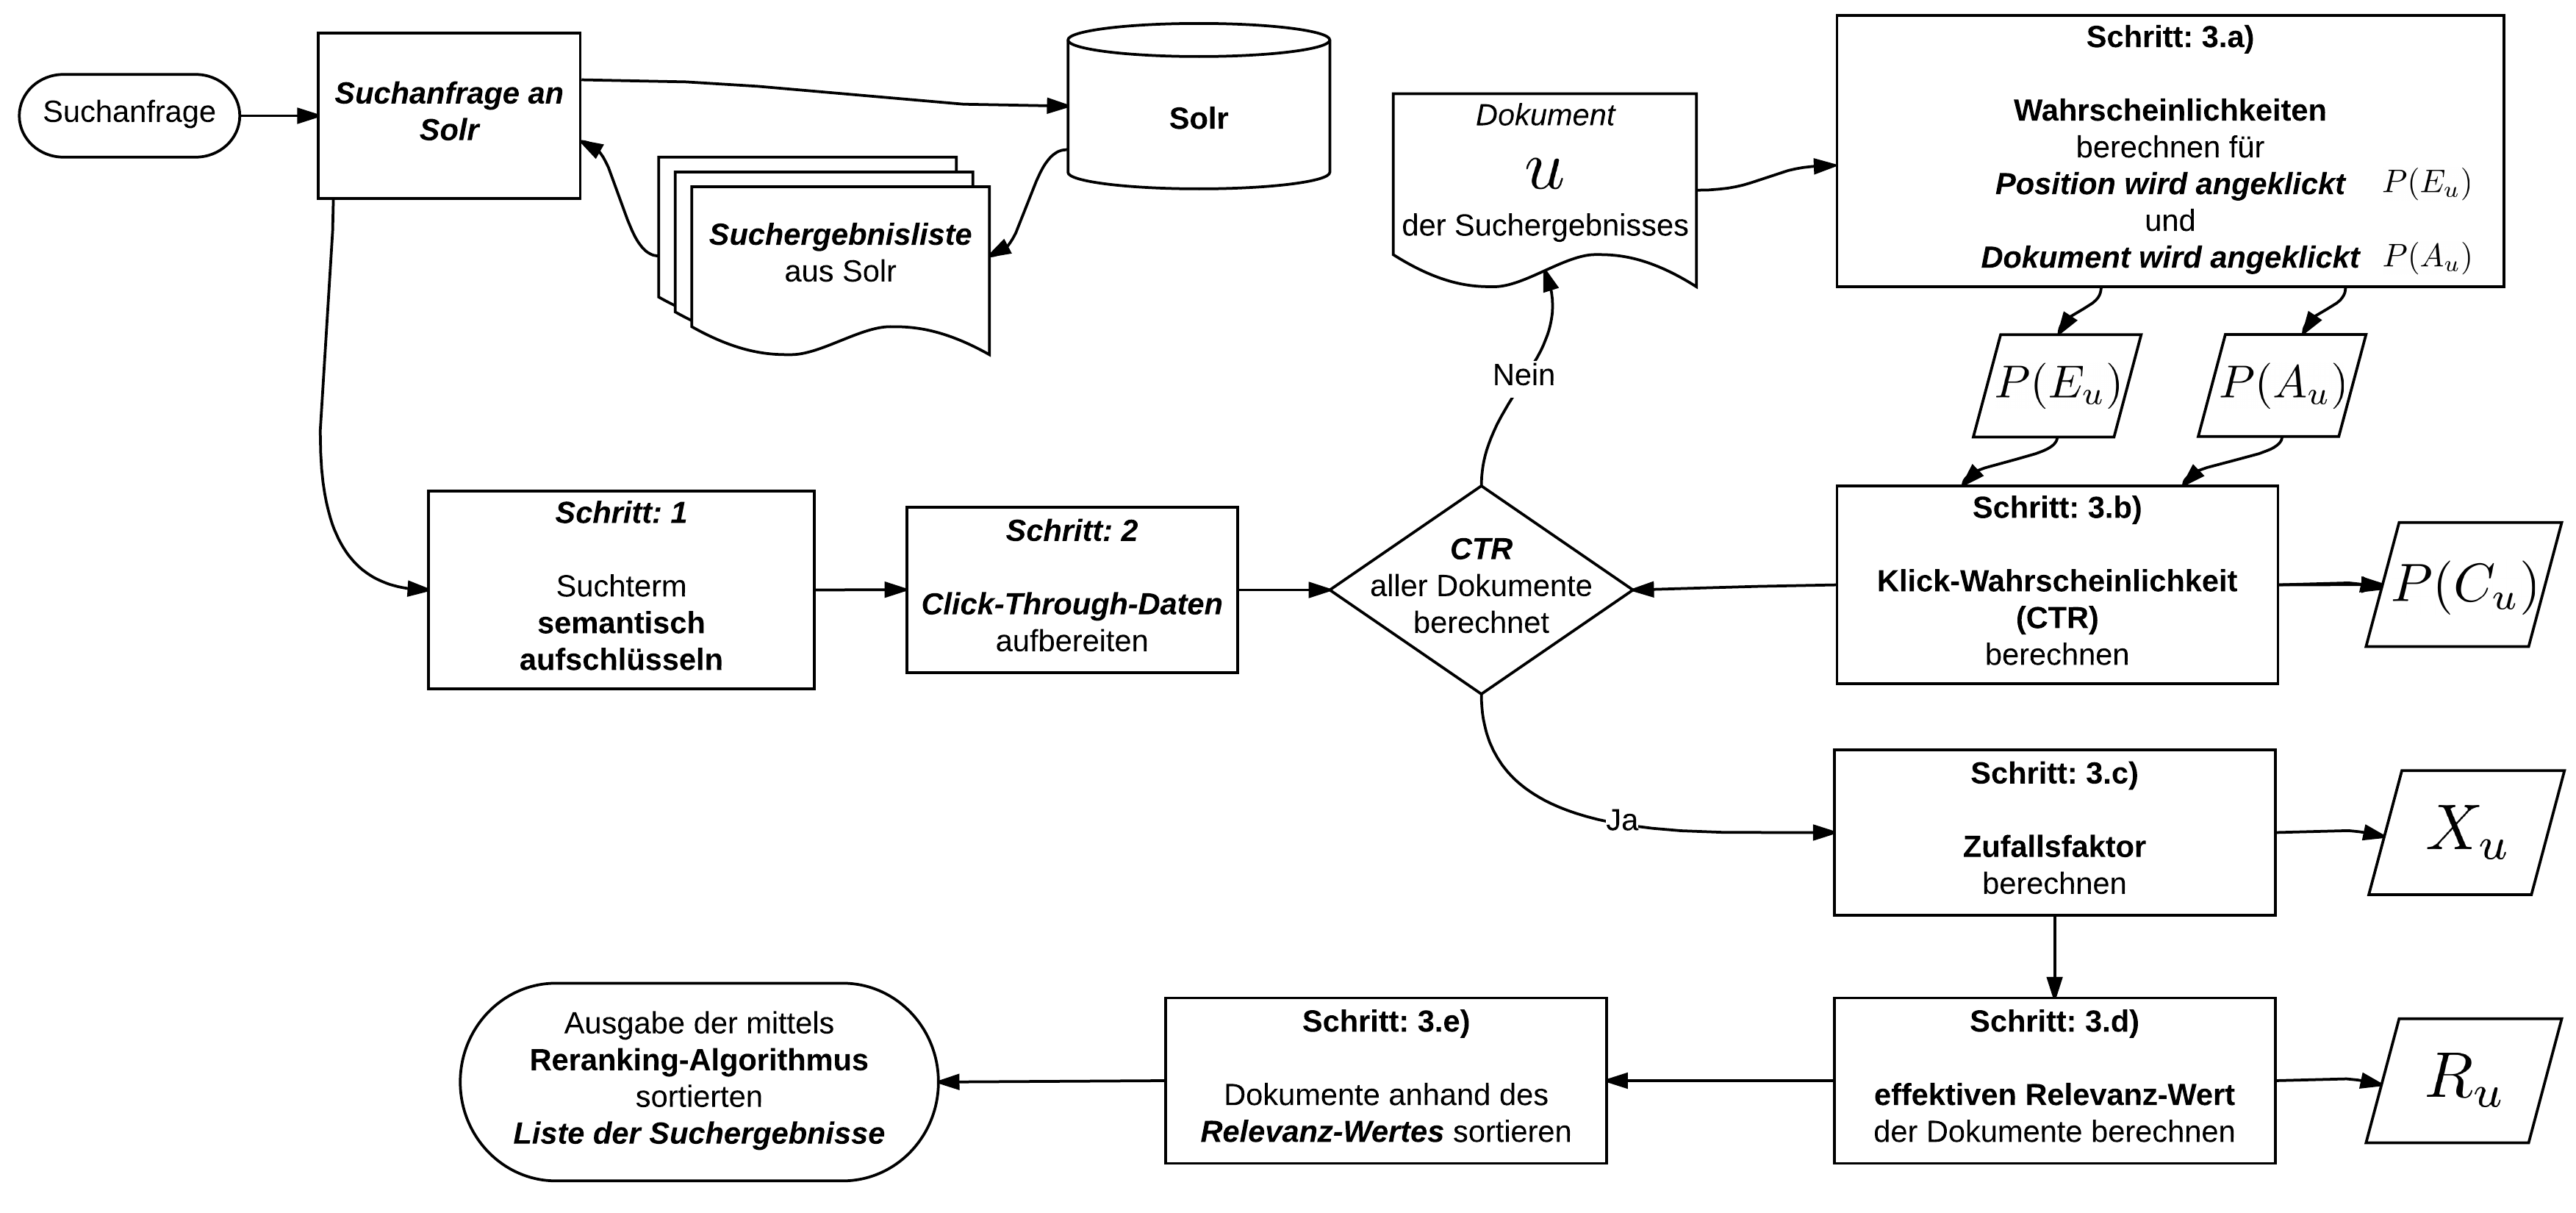
\includegraphics[width=\linewidth]{gfx/ProzessaufbauBild}
\vspace{-2em}
\end{figure}
		
%Methodik
%----------------------------------------------------------------

\section{Methodik}
\label{sec:Reranking:Methodik}

Wie bereits in der Einführung zu diesem Kapitel besprochen, haben wir gelernt wie Click-Through-Daten entstehen, wie sie zu lesen sind und wie wir Aussagen zu ihnen treffen können. Nun werden wir mithilfe dieses Wissens die CTR der Dokumente berechnen. Mithilfe der berechneten Click-Through-Daten werden wir dann ein \textit{Reranking} der Suchresultate durchführen, bevor diese dem User präsentiert werden. So wollen wir die Userrelevanz CTR in die Suche einbinden. Die Vorgehensweise dazu sieht wie folgt aus.

\subsection{Suchterm Segmentierung}
\label{sec:Reranking:Methodik:SuchtermSegmentierung}

Um alle relevanten Click-Through-Daten lesen zu können, müssen wir zunächst den Suchterm auftrennen, wie in Kapitel \ref{sec:Grundlagen:Grundbegriffe:SemantikUserInteraktionen:ProblemstellungenClick-Through-Daten} angesprochen. Der Prozess dazu sieht wie folgt aus:

\begin{figure}[H]
\centering
\vspace{-1em}
\caption[Prozess der semantischen Segmentierung des Suchterms]{Prozess der semantischen Segmentierung des Suchterms}
\label{fig:SemantischeSegmentierung}
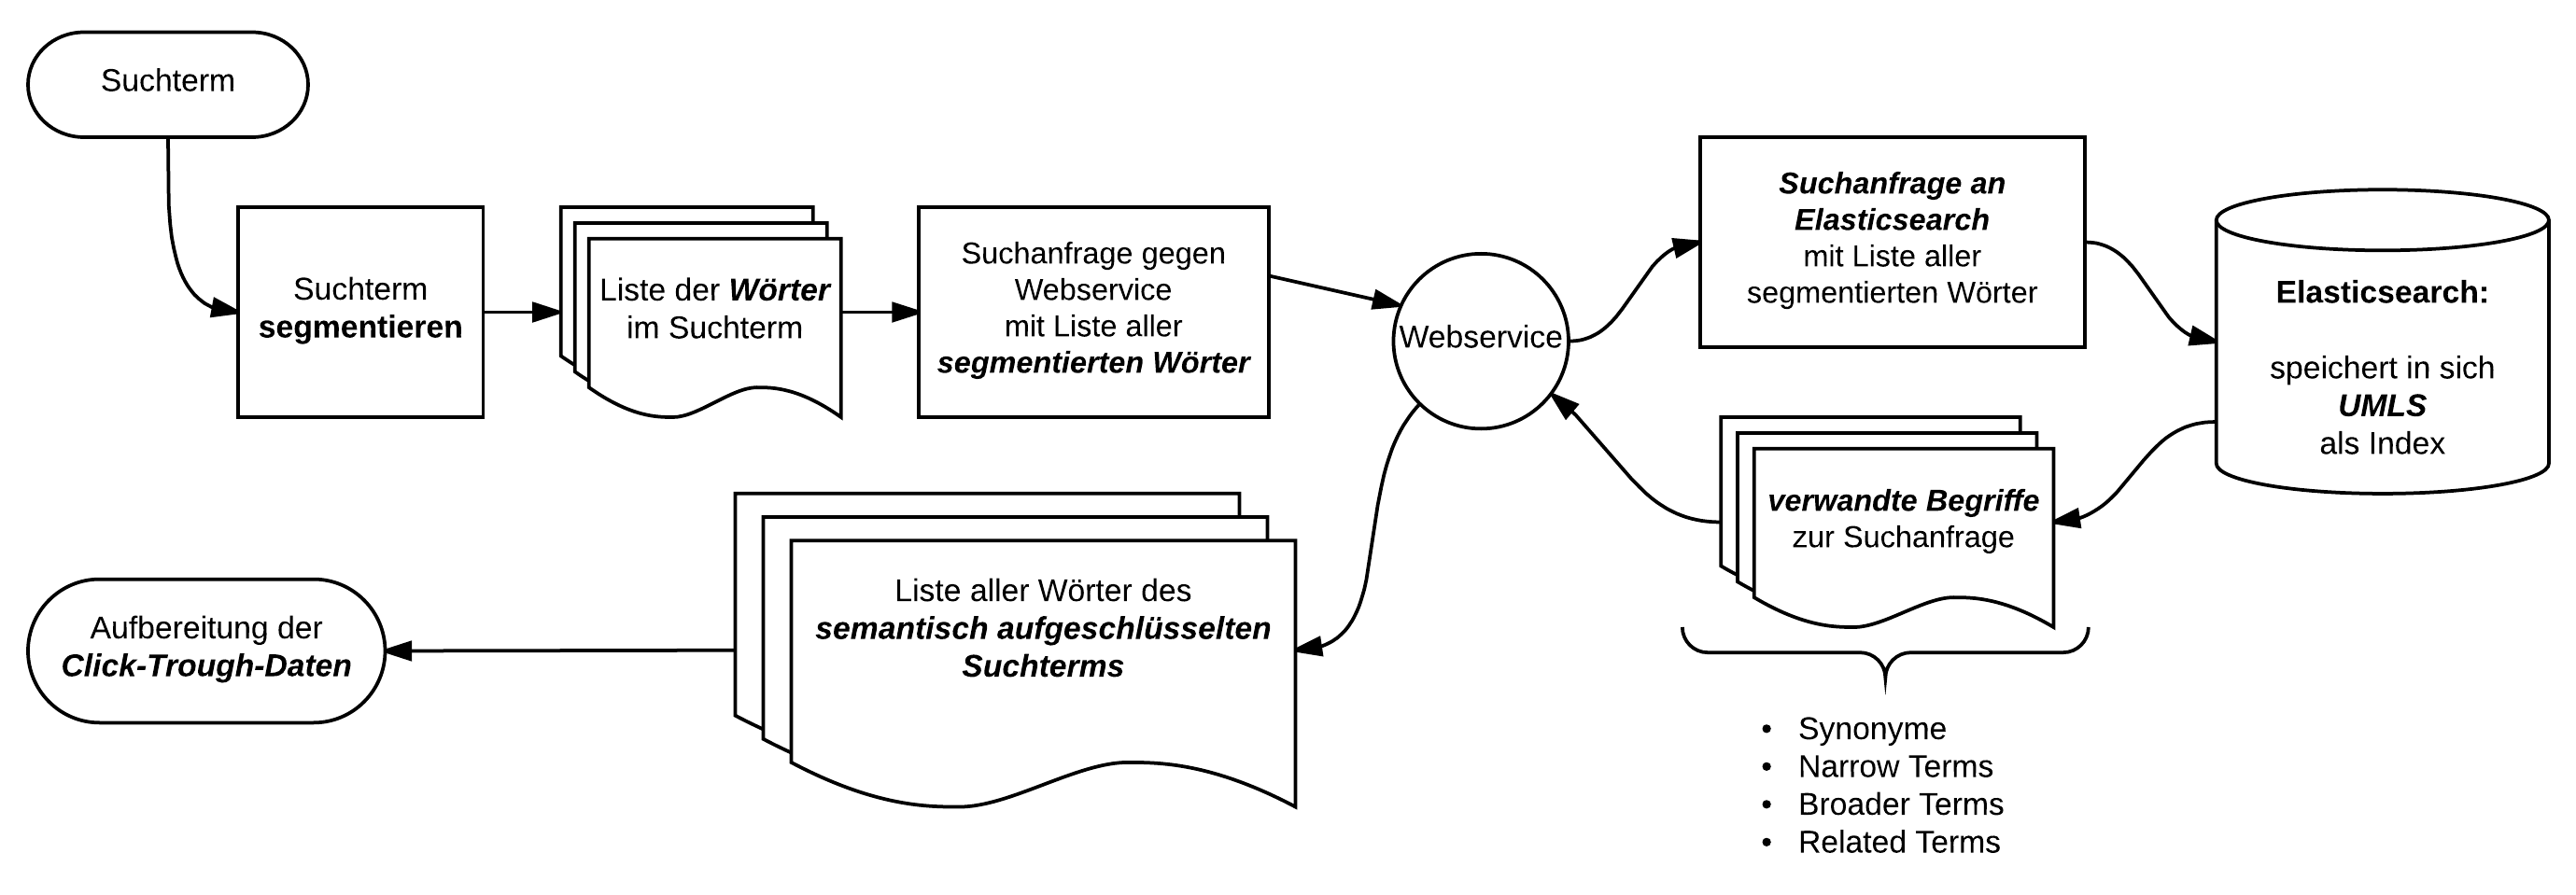
\includegraphics[width=\linewidth]{gfx/SuchtermSegmentierung}
\vspace{-2em}
\end{figure} 

\subsubsection{Suchterm semantisch aufschlüsseln mittels Segmentierung}
\label{sec:Reranking:Methodik:SuchtermSegmentierung:SuchtermSegmentierung}

Die Auftrennung des Suchterms in die einzelne Worte können wir mithilfe einer Segmentierung\footnote{Bezeichnet die Aufteilung in Abschnitte, in diesem Fall in einzelne Worte} durchführen. Hier könnten wir uns überlegen, zusätzlich mit Stoppwörtern\footnote{Stoppwörter sind Wörter, die sehr häufig auftreten und für gewöhnlich keine Relevanz für den Dokumentinhalt besitzen} nicht relevante Wörter aus dem Suchterm zu entfernen. Dieses Verfahren macht aber im Springermedizin-Kontext keinen Sinn. Wie in Kapitel \ref{sec:Einfuehrung:Problemstellung:Userrelevanz} angesprochen, suchen die User der Springermedizin-Applikation oft mit einschlägig, fundierten Fachbegriffen. Wir gehen darum davon aus, dass alle Wörter des verwendeten Suchterms für das Suchergebnis relevant sind. Diese Erkenntnis basiert auf Aussagen der Redakteure von Springermedizin und Webtrekk-Analysen der meist gesuchtesten Suchtermen der letzten Monate. Auch sind Stoppwörter veraltet und werden in modernen Information Retrieval Verfahren nicht mehr eingesetzt. Wir verzichten darum auf den Einstatz von Stoppwörtern.

\subsubsection{Suchterm semantisch erweitern mittels Thesaurus}
\label{sec:Reranking:Methodik:SuchtermSegmentierung:SuchtermThesaurus}

Wie ebenfalls in Kapitel \ref{sec:Grundlagen:Grundbegriffe:SemantikUserInteraktionen:ProblemstellungenClick-Through-Daten} thematisiert, wollen wir die Click-Through-Daten zu unserem Suchterm um Click-Through-Daten zu verwandten Begriffen erweitern. Für diese semantische Erweiterung eines Suchwortes werden wir einen Thesaurus verwenden. Die Erweiterung umfasst zum Suchterm gleichbedeutende Begriffe (\textit{Synonyme}), sehr ähnliche Begriffe (\textit{Narrow Terms}), ähnliche Begriffe im weiteren Sinne (\textit{Broader Terms}) und verwandte Begriffe (\textit{Related Terms}). 

\paragraph{Mittels Webservice einen UMLS-Thesaurus nach relevanten Begriffen durchsuchen}
Springer Nature besitzt einen Webservice mit welchem auf den Thesaurus \textit{Unified Medical Language System}~(UMLS, siehe \cite{UMLS}) zugegriffen werden kann. Der Webservice nimmt einzelne Wörter und Wörter-Listen entgegen. Zu jedem dieser Wörter durchsucht der Webservice den Thesaurus nach den oben erwähnten Arten von verwandten Begriffen. Der Webservice verwendet für diese Suche eine Elasticsearch~(siehe \cite{elasticsearch})\footnote{Eine Elasticsearch ist eine Volltextsuchmaschine}. Die dabei gefundenen Begriffe, liefert der Webservice als Antwort zurück. Um alle relevanten Click-Through-Daten zu finden, werden wir mit dem segmentierten Suchterm eine Anfrage gegen diesen Webservice stellen und anschließend den segmentierten Suchterm um die gefundenen Begriffe erweitern. Mithilfe des erweiterten Suchterms können wir dann anschließend eine Analyse in Webtrekk starten und alle relevanten Click-Through-Daten lesen. 

\subsection{Aufbereitung Click-Through-Daten}
\label{sec:Reranking:Methodik:Click-Through-Daten}

\subsubsection{Jeder Klick auf ein Dokument ist relevant}
\label{sec:Reranking:Methodik:Click-Through-Daten:Click-Through-DatenAuswertungen}

Wie in Kapitel \ref{sec:Grundlagen:Grundbegriffe:Click-Through-Daten:UserverhaltensFeedback} beschrieben, reichen Webtrekk-Analysen für komplexe Auswertungen der Click-Through-Daten nicht aus. Wir können darum in dieser Arbeit \textit{Feedback-Strategien} für die CTR Auswertung, wie in \cite{Joachims} beschrieben, nicht verwenden. Stattdessen greifen wir wie ebenfalls in Kapitel \ref{sec:Grundlagen:Grundbegriffe:Click-Through-Daten:UserverhaltensFeedback} beschrieben auf die Click-Through Features zu, die uns Webtrekk zur Verfügung stellt. Daraus entsteht das in Tabelle \ref{tab:Feature-Set} folgende, interpretierbares Feature-Set. 

\begin{table}[H]
\vspace{-.75em}
 \caption[Interpretierbares Feature-Set aus den Webtrekk Click-Through-Daten]{Interpretierbares Feature-Set aus den Webtrekk Click-Through-Daten}
\label{tab:Feature-Set}
\vspace{-.5em}
\footnotesize
\renewcommand*{\arraystretch}{1.2}
\resizebox{\textwidth}{!}{%
\begin{tabular}{ll}
\hline
\multicolumn{2}{l}{\textit{\textbf{Click-Through Features}}}                                                                      \\ \hline
\textbf{Feature}          & \textbf{Beschreibung}                                                                                 \\ \hline
\textit{Position}         & Position dieses Dokumentes im Suchergebnis (angeklickte Position)                                     \\
\textit{ClickFrequency}   & Anzahl Klicks für dieses Dokument zum angefragten Suchterm (Klick-Häufigkeit)                         \\
\textit{ClickProbability} & Klick-Wahrscheinlichkeit zum Suchterm (ClickFrequency / Gesamtanzahl Klicks zum angefragten Suchterm) \\ \hline
\end{tabular}
}
\vspace{-2em}
\end{table}

Wie wir sehen können ist unser Feature-Set im Vergleich zu dem in \cite{IWUSBI} beschriebenen sehr stark eingeschränkte und enthält keine Informationen um ein Relevanz-Feedback zu den Klick-Häufigkeiten daraus lesen zu können. Wir müssen wir darum davon ausgehen, dass jeder Klick auf ein Dokument relevant ist.

\subsubsection{Gewichtung der Click-Through-Daten}
\label{sec:Reranking:Methodik:Click-Through-Daten:Gewichtung}

Durch die semantische Aufschlüsselung des Suchterms haben wir verschieden starke Relationen zwischen Click-Through-Daten und dem Suchterm. Die Gewichtung der Stärke dieser Relation ist aber nicht Kern dieser Arbeit. Wir gehen darum davon aus, dass unabhängig der stärke der Relation zum Suchterm, alle Click-Through-Daten eine gleiche Relevanz besitzen.

\subsubsection{Berechnung der CTR}
\label{sec:Reranking:Methodik:Click-Through-Daten:Gewichtung}

\paragraph{Einfache CTR ignoriert viele Problemstellungen der Interaktion der User mit der Suche} 
Wie wir bereits wissen, stellt die CTR die Anzahl der Klicks auf ein Dokument im Verhältnis zu den gesamten Impressionen dar. Bezogen auf das in Kapitel \ref{sec:Grundlagen:Grundbegriffe:Click-Through-Daten:UserverhaltensFeedback} angesprochene Feature-Set, würden wir die \textit{ClickProbability} direkt als CTR verwenden. Dazu müssten wir nur die Click-Through-Daten eines Dokuments ins Verhältnis zu allen Click-Through-Daten für einer Suchanfrage stellen. Wie wir aber bereits in Kapitel \ref{sec:Grundlagen:Grundbegriffe:SemantikUserInteraktionen:ProblemstellungenClick-Through-Daten} gelernt haben, würden wir damit viele Problemstellungen der Interaktion der User mit der Suche ignorieren. Deswegen haben wir uns für eine Lösung basierend auf einem Klick-Modell entschieden. 

\paragraph{Klick-Wahrscheinlichkeit als CTR für Reranking verwenden} 
Klick-Modelle versuchen die Click-Through-Daten zu interpretieren und aus ihnen ein Relevanz-Feedback zu schlussfolgern. Das machen sie mithilfe des bereits angesprochenen Feature-Set der Click-Through-Daten. Aus dem Feature-Set von Springermedizin können wir zwei wichtige Informationen zu jeder Suchanfrage ermitteln. Wir wissen welches Dokument auf welcher Position im Suchresultat angeklickt worden ist und wir kennen die Reihenfolge der Dokumente im Suchresultat der Solr. Der \textit{PBM} basierte Algorithmus baut genau auf diesen Click-Through-Informationen auf und berechnet daraus eine Klick-Wahrscheinlichkeit, welche wir anstelle der einfachen CTR für das Reranking der Suchergebnisliste verwenden können. 

\subsection{Result-Reranking mittels PBM basiertem Algorithmus}
\label{sec:Reranking:Methodik:Result-RerankingPBM}

\subsubsection{Click-Through-Daten für Positions- und Dokument-Wahrscheinlichkeit abfragen}
\label{sec:Reranking:Methodik:Result-RerankingPBM:PositionDokumentWahrscheinlichkeiten}

In Kapitel \ref{sec:Grundlagen:Grundbegriffe:Result-RerankingPBM:Grundlagen} haben wir gelernt, dass sich das PBM aus der Dokument-Wahrscheinlichkeit $P(A_{u})$ und der Positions-Wahrscheinlichkeit $P(E_{r_u})$ zusammensetzt. Die dabei vorgestellten Formeln zur Berechnung der beiden Wahrscheinlichkeiten verwenden unterschiedliche Click-Through-Daten. Der Prozess für das Lesen der relevanten Click-Through-Daten sieht wie folgt aus:

\begin{figure}[H]
\centering
\vspace{-1em}
\caption[Click-Through-Daten für Wahrscheinlichkeitswerte lesen]{Click-Through-Daten für Wahrscheinlichkeitswerte lesen}
\label{fig:WahrscheinlichkeitswerteCTDaten}
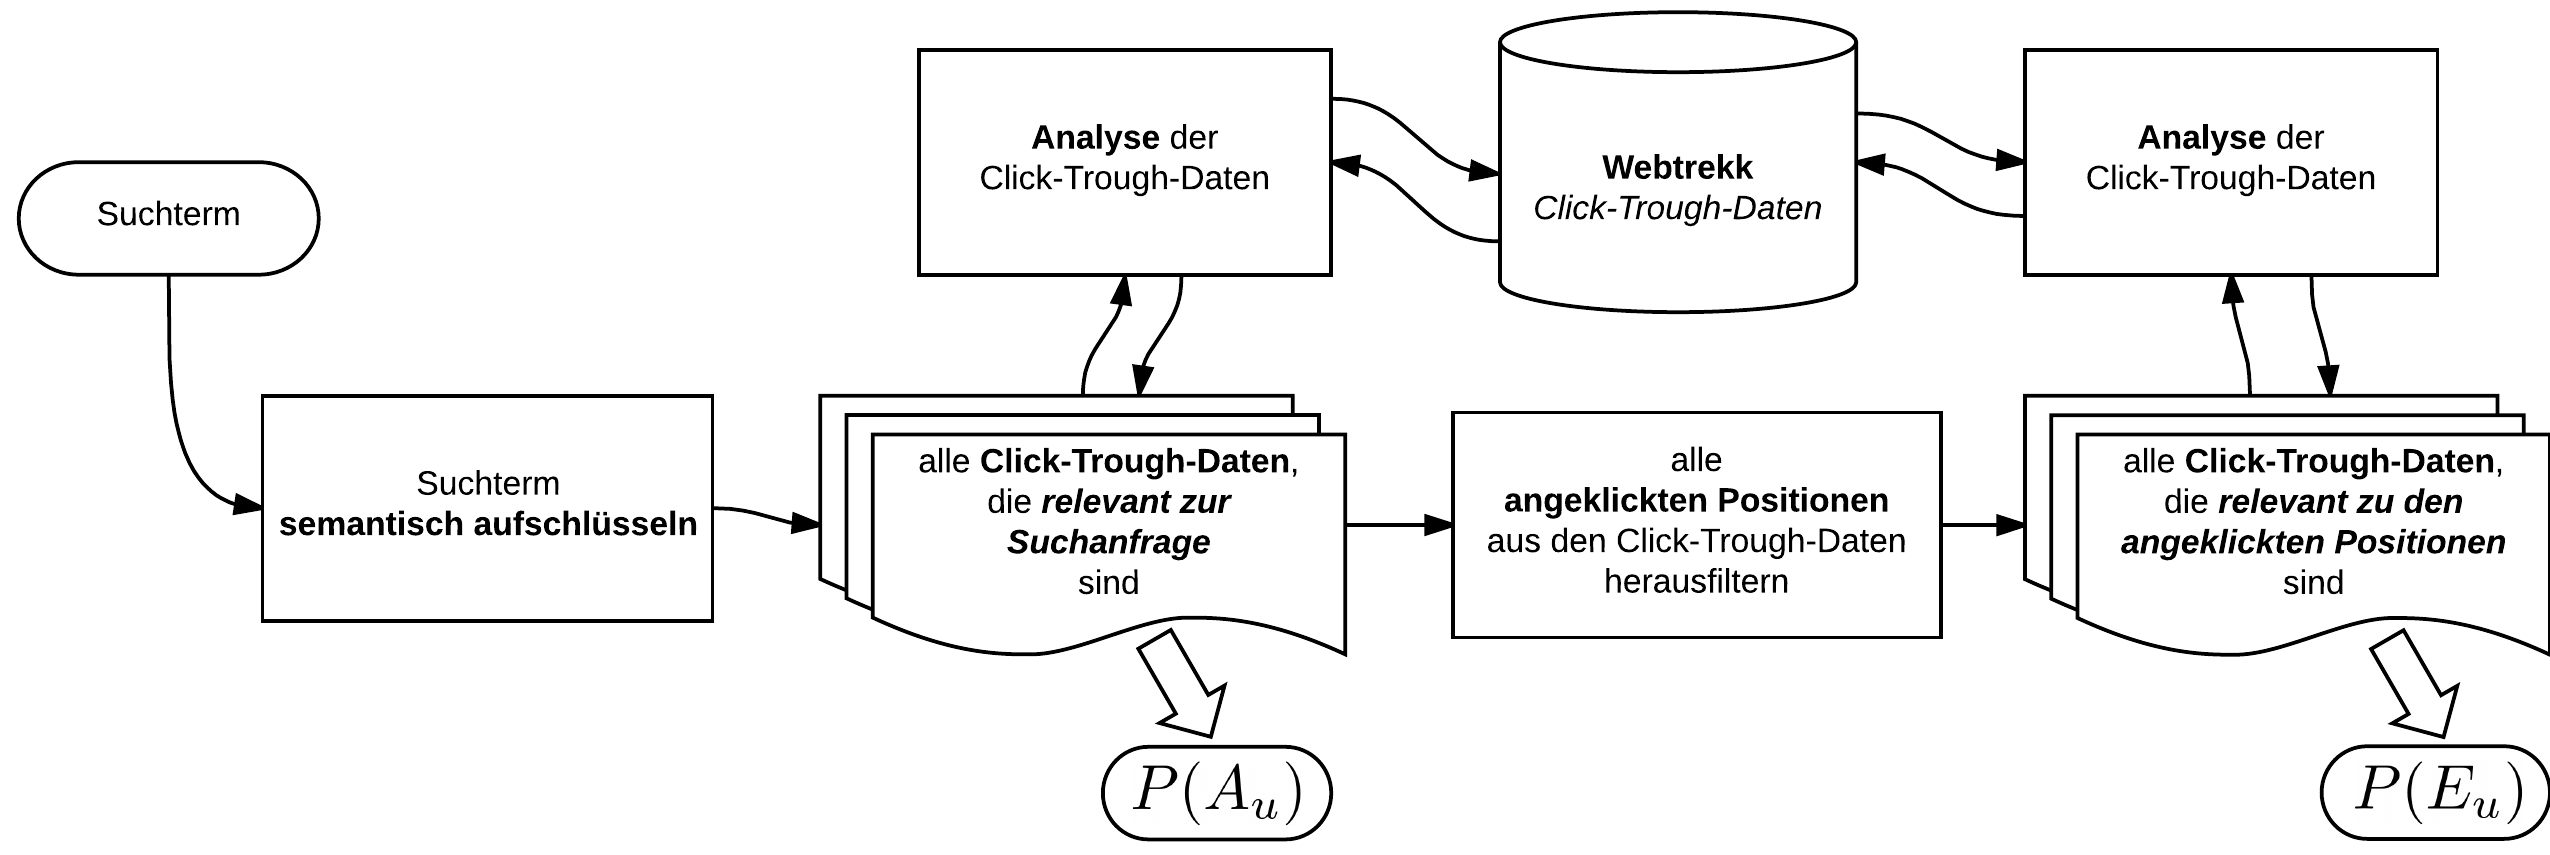
\includegraphics[width=\linewidth]{gfx/WahrscheinlichkeitswerteCTDaten}
\vspace{-2.5em}
\end{figure}

\paragraph{Click-Through-Daten der Dokument-Wahrscheinlichkeit $P(A_{u})$ filtern}
Für die Berechnung der Dokument-Wahrscheinlichkeit verwenden wir das weiter oben in Kapitel \ref{sec:Reranking:Methodik:Click-Through-Daten:Click-Through-DatenAuswertungen} angesprochene Verfahren zur Suchterm-Segmentierung, um \textit{alle für die Suchanfrage relevanten Click-Through-Daten} zu lesen. Aus diesen Click-Through-Daten können wir dann mithilfe der vorgestellten Formel für $P(A_{u})$ die Wahrscheinlichkeit berechnen, dass ein Dokument aufgrund seines Suchsnippets im Suchergebnis angeschaut wird.  

\paragraph{Click-Through-Daten der Positions-Wahrscheinlichkeit $P(E_{u})$ filtern}
Für die Berechnung der Positions-Wahrscheinlichkeit filtern wir aus den für die Dokument-Wahrscheinlichkeit
gelesenen Click-Through-Daten \textit{alle angeklickten Positionen} heraus. Zu diesen Positionen lesen wir dann unabhängig des Suchterms, alle Click-Through-Daten in denen auf diese Positionen geklickt wurde. Aus den resultierenden Click-Through-Daten können wir dann mithilfe der vorgestellten Formel für $P(E_{r_u})$ die Wahrscheinlichkeit berechnen, dass ein Dokument aufgrund aufgrund seiner Position im Suchergebnis angeschaut wird.

\subsubsection{Klick-Wahrscheinlichkeit mit PBM berechnen}
\label{sec:Reranking:Methodik:Result-RerankingPBM:Klick-Wahrscheinlichkeit}

Wie in Kapitel \ref{sec:Grundlagen:Grundbegriffe:Result-RerankingPBM:AnsatzSucheEinbinden} angesprochen, werden wir unseren Reranking-Algorithmus in die Aufbereitung der Suchresultate aus der Solr-Suche integrieren. Wir werden die Click-Through-Daten wie im vorherigen Teil der Methodik besprochen aufbereiten und dann darauf unseren Reranking-Algorithmus anwenden um die CTRs der einzelnen Dokumente des Suchergebnisses zu berechnen. 

\paragraph{Reranking-Algorithmus kann nur die Top-N-Ergebnisse betrachten}
Wir müssen bei unserem Ansatz beachten, dass die Solr durch die Pagination-Funktion~(siehe \cite{Pagination}) nur die Top-N-Ergebnisse zurückgibt. Dadurch sehen wir nur einen Teil der Suchergebnisse. Um sicherzustellen, dass wir möglichst viele relevante Suchergebnisse berücksichtigen, werden wir die ersten 100 Suchergebnisse der Solr im Reranking-Algorithmus verarbeiten. Aus der daraus resultierenden Liste der Suchergebnisse, filtern wir die ersten 20 Ergebnisse und stellen diese dar. Für die Untersuchung des Reranking-Algorithmus werden wir uns bei der Auswertung jeweils auf die Seite 1 der Suchergebnisse konzentrieren. Bei Springermedizin somit auf die ersten 20 Suchresultate. Die Pagination der Folgeseiten der Suchresultate werden wir nicht untersuchen. Würden wir diesen Algorithmus in einer Live-Applikation\footnote{Mit Live-Applikation wird hier eine öffentliche, für Kunden zugängliches Applikation beschrieben} implementieren wollen, müssten wir uns für die Ausspielung der Folgeseiten des Suchresultats zusätzlich einen Lösungsansatz überlegen, damit die Solr die durch den Reranking-Algorithmus bereits ausgespielten Suchresultate nicht mehrfach ausspielt.

\paragraph{Ausarbeitung des effektiven Algorithmus}
Unseren Reranking-Algorithmus bauen wir auf der in Kapitel \ref{sec:Grundlagen:Grundbegriffe:Result-RerankingPBM:Grundlagen} vorgestellten Formel des PBMs auf. Wie wir in der Analyse der Grundlagen in Kapitel \ref{sec:Grundlagen:Grundbegriffe} festgestellt haben, reicht die triviale Umsetzung unseres Klick-Modells für unseren Algorithmus nicht aus. Wir haben darum verschiedene Lösungsansätze für die Problemstellungen vorgestellt. Mithilfe einiger dieser Lösungsansätzen, wollen wir nun den effektiven Algorithmus ausarbeiten.

\subsubsection{Smoothing-Faktor in PBM einführen}
\label{sec:Reranking:Methodik:Result-RerankingPBM:SmoothingPBM}

Wir wissen dass eine Wahrscheinlichkeit einen Wert zwischen 0 und 1 besitzt. Dadurch können Nullwerte entstehen. Das PBM multipliziert die Positions- und Dokument-Wahrscheinlichkeit miteinander, um die Klick-Wahrscheinlichkeit zu berechnen. Wir müssen aber davon ausgehen, dass es Dokumente im Suchresultat geben kann, deren Position nie angeklickt worden ist und umgekehrt. Multiplikationen mit Null ergeben immer einen Nullwert.  Wir führen darum an dieser Stelle einen \textit{Smoothing-Faktor} ein:

\begin{figure}[H]
\centering
\vspace{-1em}
\caption[Berechnung der CTR mittels PBM]{Berechnung der CTR mittels PBM}
\label{fig:BerechnungCTRmittelsPBM}
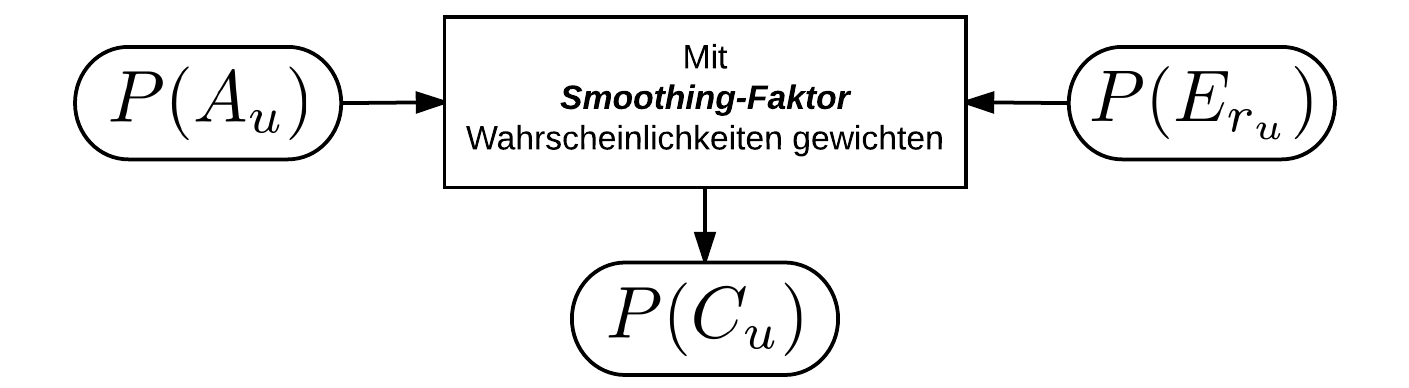
\includegraphics[width=.5\linewidth]{gfx/BerechnungCTRmittelsPBM}
\vspace{-2.5em}
\end{figure}

\paragraph{Mit Smoothing-Faktor Wahrscheinlichkeitswerte gewichten}
Der Smoothing-Faktor soll zwei Probleme lösen. Zum Einen wollen wir einen Wahrscheinlichkeitswert trotz der Multiplikation mit Null beachten (1). Zum Anderen wollen wir die im vorherigen Absatz beschriebene Gewichtung abhängig des Relevanz-Feedbacks in den Algorithmus einbeziehen (2). Wir transformieren dazu das Produkt der beiden Wahrscheinlichkeiten in eine gewichtete Summe indem wir eine \textit{Smooting-Konstante} einführen. Die Smoothing-Konstante $\lambda$ soll die Gewichte der beiden Klick-Wahrscheinlichkeiten $P(E_{r_u})$ und $P(A_{u})$ zu eins aufsummieren. Wir verwenden dazu das \textit{Exponential Smoothing Modell}~(siehe \cite{ExpSmoothing}). Bilden wir dieses Modell auf den PBM basierten Algorithmus ab, sieht die Formel für die CTR (CTR = $P(C_{u})$) wie folgt aus:
  
\vspace{-1.5em}
\begin{equation}
	P(C_{u}) = \lambda\cdot P(E_{r_u}) + (1 - \lambda)\cdot P(A_{u})
\end{equation}
\vspace{-1.5em}

\subsubsection{Smoothing-Faktor abhängig der Position im Suchresultat definieren}
\label{sec:Reranking:Methodik:Result-RerankingPBM:VerhaeltnisKlick-Wahrscheinlichkeiten}

Die in Kapitel \ref{sec:Grundlagen:Grundbegriffe:Result-RerankingPBM:Grundlagen} angesprochene Studie \cite{pbm} hat aufgezeigt, dass das PBM sich stark an der Position eines Dokumentes im Suchresultat orientiert und dies negative Einflüsse auf die Prognose der CTR haben kann. Die Klick-Wahrscheinlichkeit $P(E_{r_u})$ darf darum nicht zu viel Einfluss haben. Aus eigener Erfahrung wissen wir zudem, dass die ersten Dokumente im Suchresultat immer zuerst gesehen werden. Die dahinter gelisteten Dokumente werden fortlaufend analysiert. Dies bestätigt die in Abb. \ref{fig:Grundlage:AnalyseKlicksPositionen} dargestellte Analyse der Klicks auf die ersten 20 Positionen eines Suchergebnisses. Wir sollten darum darauf achten, dass je \textit{schlechter} die Position des angeklickten Dokumentes im Suchresultat der Solr ist, desto \textit{höher} das Relevanz-Feedback zu bewerten ist. 
\\
\\
Das machen wir, indem wir für die Berechnung der CTR des Dokumentes den Smoothing-Faktor abhängig der Position im Suchresultat definieren. Dadurch können wir das Verhältnis zwischen Klick-Wahrscheinlichkeit der Position und Klick-Wahrscheinlichkeit des Dokumentes steuern. Als Grundlage hierbei dient uns die Position des Suchresultats der Solr. Wie die Aufteilung dazu aussehen wird, sehen wir folgend:

\begin{table}[H]
\centering
\vspace{-.75em}
 \caption[Smoothing-Faktor abghängig der Position im Suchergebnis]{Smoothing-Faktor abghängig der Position im Suchergebnis}
\label{tab:VerhaeltnisKlick-WahrscheinlichkeitenPositionDokument}
\vspace{-.5em}
\footnotesize
\renewcommand*{\arraystretch}{1.2}
\begin{tabular}{lcc} \hline
	\textbf{Position} & \textbf{Verhältnis Position zu Dokument} & \textbf{Wert des Smoothing-Faktors $\lambda$}\\ \hline
	1 bis 10 & 1:1 & 0.50\\ \hline
	11 bis 20 & 1:2 & 0.34\\ \hline
	größer 20 &  1:3 & 0.25\\ \hline
 \end{tabular}
\vspace{-2em}
\end{table}

Für die Suchresultate mit einer Position über 20, verstärken wir die Gewichtung der Klick-Wahrscheinlichkeit des Dokumentes erheblich. Wir gehen davon aus, dass bei Klicks auf Dokumente mit einer solch hohen Position, die suchende Person die Suchresultate genau analysierte, bevor sie ein Dokument angeklickt hat.

\subsection{Vergessen der alten Daten}
\label{sec:Reranking:Methodik:Vergessen}

Ein Algorithmus zur Berechnung von Wahrscheinlichkeiten muss sich ein gewisses Grundwissen aneignen. Dies geschieht üblicherweise durch Trainingsdaten. Genauso muss er alte Daten wieder vergessen können, um Overfitting\footnote{Überanpassung des Algorithmus durch zu viele (falsche oder veraltete) Daten} zu vermeiden. 

\subsubsection{Durch Webtrekk ist kein komplexer Lern-Algorithmus notwendig}
\label{sec:Reranking:Methodik:Vergessen:Lern-Algorithmus}

Durch Webtrekk haben wir eine Wissensbasis, die sich stetig und zeitnah aktualisiert. So muss der Algorithmus nicht stetig neues Wissen lernen und altes vergessen, sondern er kann direkt diese Wissensbasis zugreifen. Dies geschieht, indem zur Laufzeit\footnote{Unter Laufzeit wird in diesem Fall der Zeitpunkt der direkte Abfrage während der Suchanfrage bezeichnet} Analysen gegen Webtrekk über eine frei definierbare Periode gemacht werden. Dadurch kann \textit{Overfitting} vermieden werden. Deshalb verwenden wir keinen komplexen Lern-Algorithmen wie in \cite{IWUSBI} vorgestellt.

\subsubsection{Die Klick-Wahrscheinlichkeit ist kein absoluter Wert für die Userrelevanz}
\label{sec:Reranking:Methodik:Vergessen:Relevanzfeedback}

Nun könnten wir die Klick-Wahrscheinlichkeit als absoluten Wert für die \textit{Userrelevanz} betrachten. Dies wäre jedoch falsch, wie in Kapitel \ref{sec:Grundlagen:Grundbegriffe:SemantikUserInteraktionen:RankExamination} analysiert, müssen wir davon ausgehen, dass viele User der Qualität der Suchmaschine vertrauen. Diese betrachten die \glqq Top-Suchresultate\grqq{} als die relevanten Suchresultate. Denkbar wäre auch, dass User unabsichtlich das falsche Dokument anklicken und dadurch die CTR eines Dokumentes verfälschen. Dadurch kann ein \textit{Overfitting} des Algorithmus entstehen.

\subsubsection{Overfitting vermeiden}
\label{sec:Reranking:Methodik:Vergessen:Overfitting}

Um ein Overfitting zu vermeiden, darf der Algorithmus nicht immer anschlagen. Wir müssen sicherstellen, dass vereinzelt \textit{zufällige Dokumente} in den \glqq Top-Suchresultaten\grqq{} angezeigt werden. So können auch andere Dokumente in den Fokus des Users gerückt werden. Das System fährt sich dadurch nicht auf falschen Annotationen fest. 

\paragraph{Zusätzliche Varianz durch Zufallsfaktor} 
Mithilfe eines Zufallsfaktors kann eine solche Varianz\footnote{Mit Varianz bezeichnen wir hierbei eine Abweichung vom berechneten Erfahrungswert} in den Klick-Modell basierten Algorithmus gebracht werden. Konkret wollen wir den Reranking-Algorithmus beeinflussen, indem wir mithilfe eines Zufallsfaktors, Abweichungen von der berechneten Klick-Wahrscheinlichkeit eines Dokumentes provozieren. Den dazu verwendeten Zufallswert $X_{u}$  lassen wir uns als positive ganze Zahl generieren. Sie soll eine Zufallsposition im Suchergebnis darstellen:

\vspace{-1.5em}
\begin{equation}	
	X_{u} \in \lbrace \text{Positionen im Suchresultat} \rbrace \subset \mathbb{N}
\end{equation}
\vspace{-1.5em}

\subsubsection{Zufallsfaktor mittels Smoothing-Faktor in 	die Sortierung der Suchergebnisse einbauen}
\label{sec:Reranking:Methodik:Vergessen:ZufallsfaktorSmoothing}

Mit unserem berechneten Zufallswert können wir nun die angesprochenen Abweichungen in die Klick-Wahrscheinlichkeiten der Dokumente einbauen. Wie bereits in Kapitel \ref{sec:Grundlagen:Grundbegriffe:SemantikUserInteraktionen:DocumentAttraction} und \ref{sec:Grundlagen:Grundbegriffe:SemantikUserInteraktionen:RankExamination} thematisiert, werden viele Suchresultate nie und deren Position selten bis gar nicht angeklickt. Sie haben darum keine Click-Through-Daten. Deren Klick-Wahrscheinlichkeit ist entweder Null oder sehr klein. Der Zufallswert soll darum nur leichte Einflüsse in die Klick-Wahrscheinlichkeit haben.

\paragraph{Effektive Position im Suchergebnis mittels Smoothing-Faktor berechnen} 
Ein direkter Einbau in die Klick-Wahrscheinlichkeitsberechnung ist jedoch schwierig, da die Wahrscheinlichkeitsverteilungen auf die Dokumente im Suchergebnis stark schwanken und sich der Einfluss des Zufallswertes dadurch stetig verändert. Wir werden darum die Klick-Wahrscheinlichkeit und den Zufallswert der Dokumente separat verarbeiten und zum Schluss die zwei daraus resultierenden Werte eines Dokumentes, mithilfe eines Smoothing-Faktors gewichtet aufsummieren. Diese Summe dient dann als Relevanz-Wert eines Dokumentes. Das Reranking der Dokumente werden wir anhand dieser Relevanz-Werte durchführen. Die Verarbeitung sieht wie folgt aus:

\begin{figure}[H]
\centering
\vspace{-1em}
\caption[Berechnung der effektiven Position im Suchergebnis mittels Smoothing-Faktor]{Berechnung der effektiven Position im Suchergebnis mittels Smoothing-Faktor}
\label{fig:BerechnungRerankedPosition}
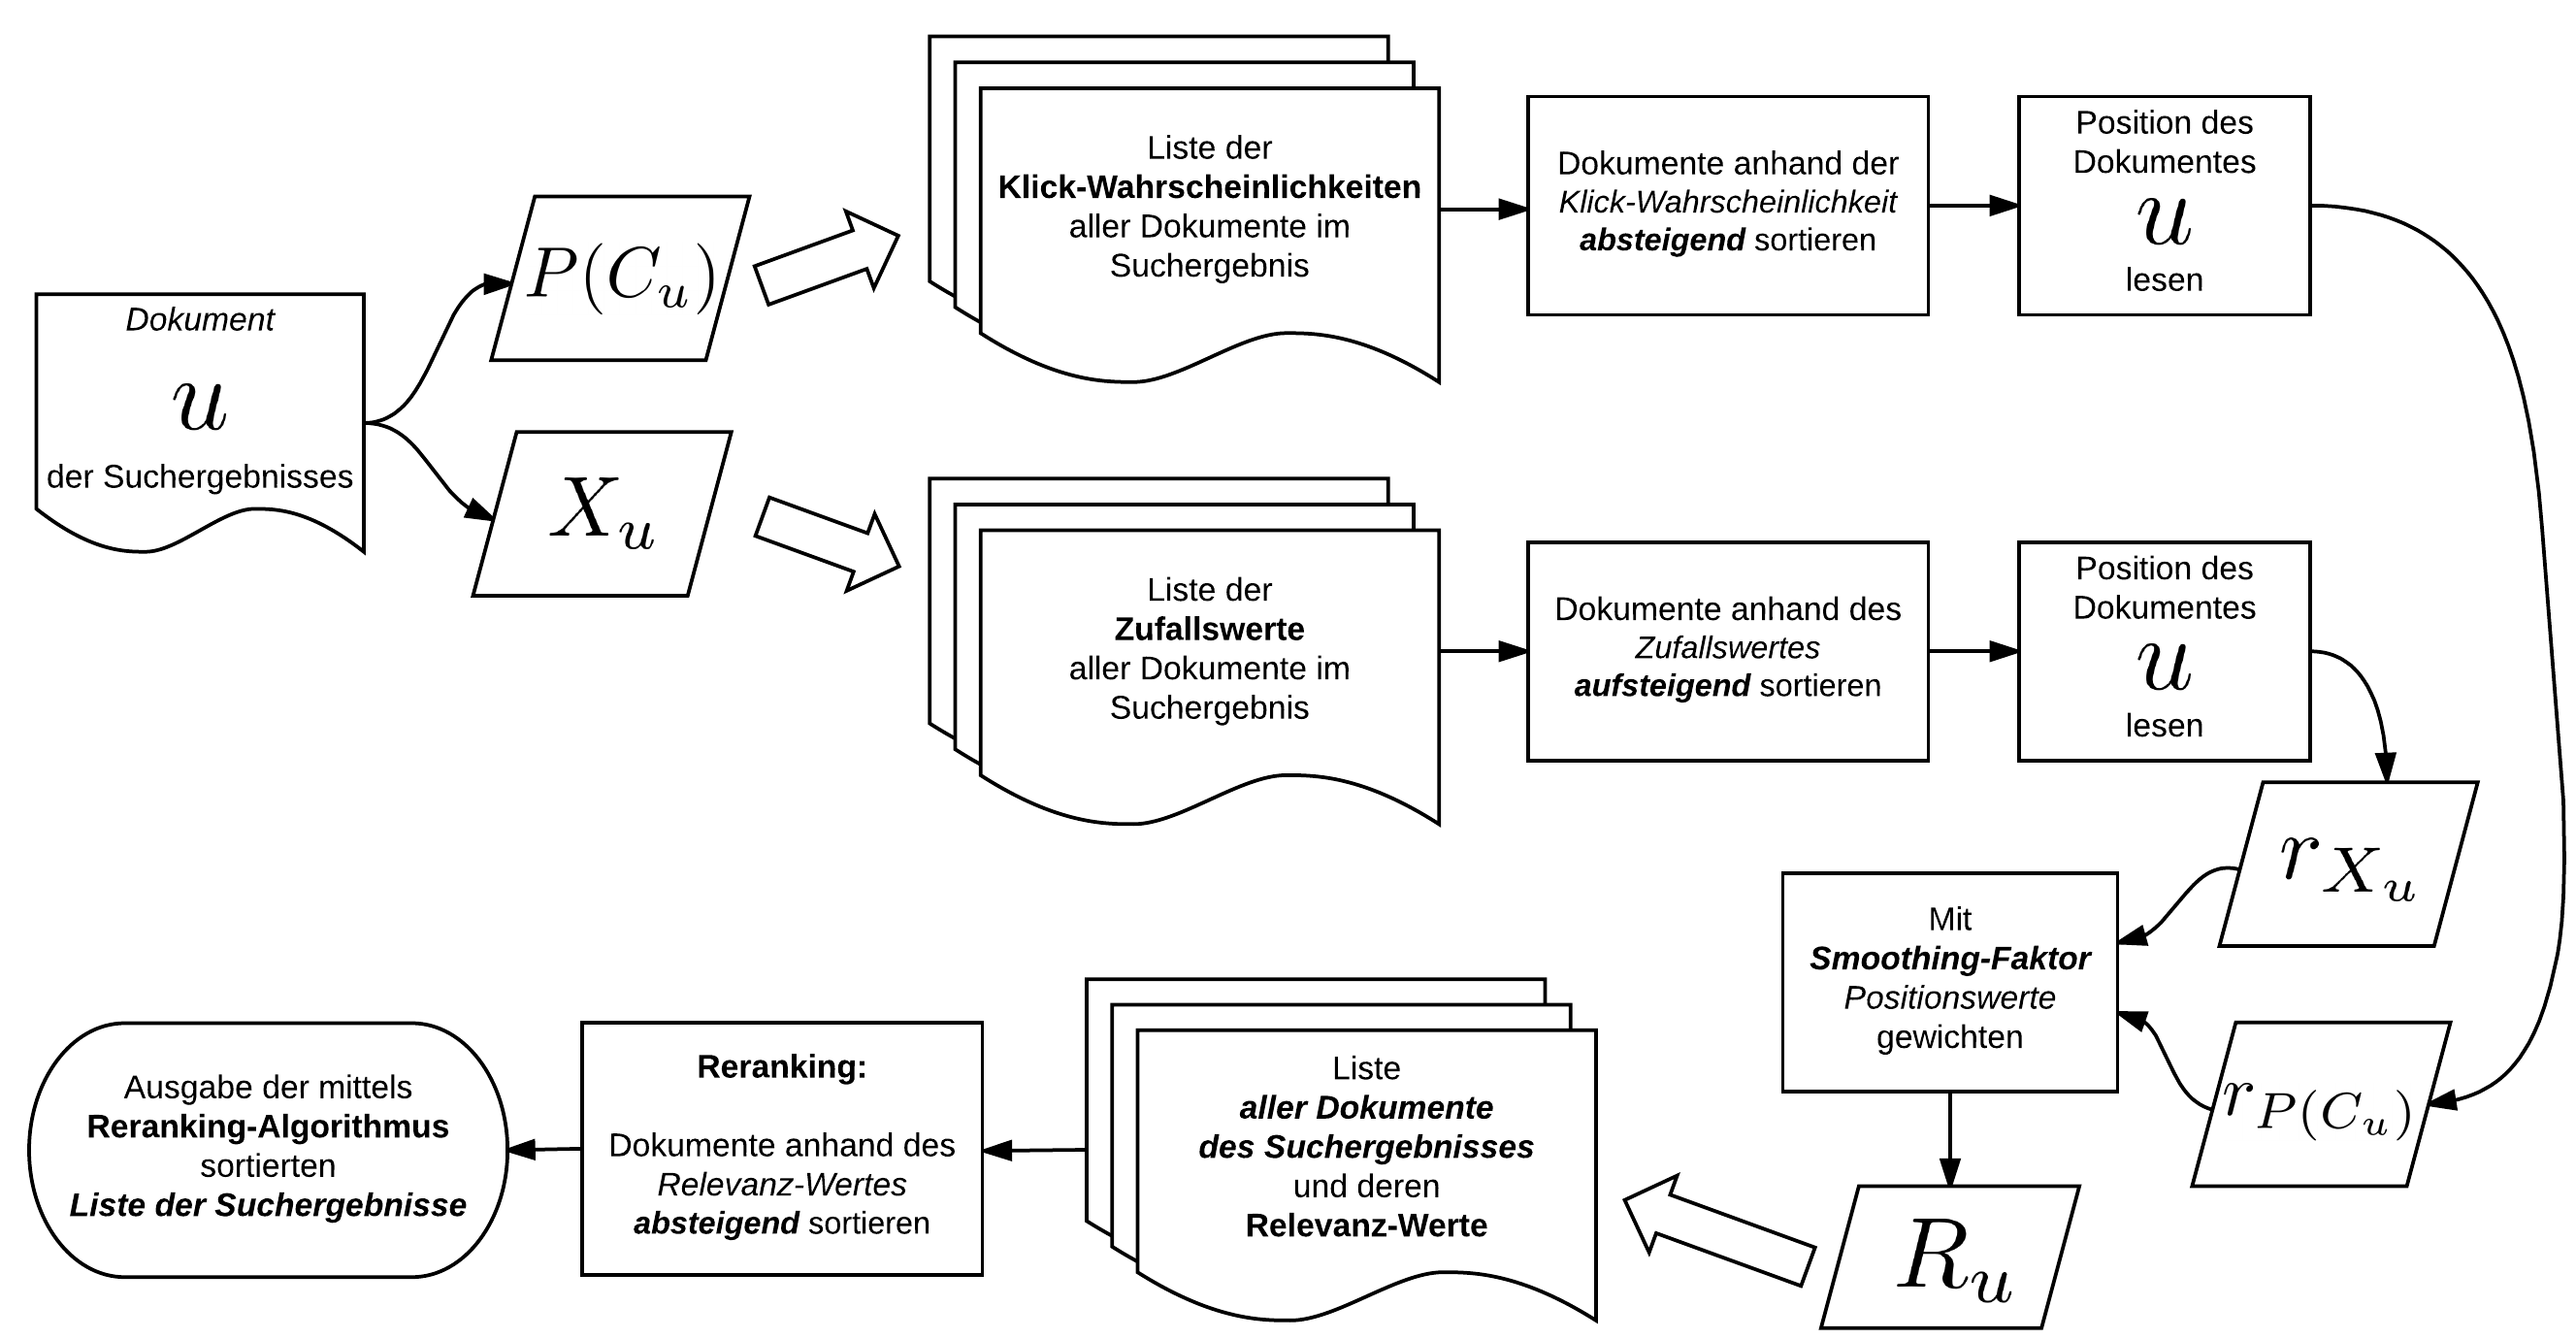
\includegraphics[width=\linewidth]{gfx/BerechnungRerankedPosition}
\vspace{-2.5em}
\end{figure}

Aus den Klick-Wahrscheinlichkeiten und den Zufallswerten der Dokumente des Suchergebnisses erzeugen wir zwei Listen und sortieren diese wie in der Abbildung beschrieben. Aus diesen Listen können wir für jedes Dokument $u$ jeweils eine Position aus der Liste der Klick-Wahrscheinlichkeiten $r_{P(C_{u})}$ und eine Position aus der Liste der Zufallswerte $r_{X_{u}}$ lesen. Aus diesen beiden Positionswerten des Dokumentes berechnen wir den effektiven Relevanz-Wert des Dokumentes $R_{u}$. Dazu verwenden wir wieder das \textit{Exponential Smoothing Modell} für den Smoothing-Faktor und berechnen damit die gewichtete Summe der beiden Positionswerte. Wie bereits weiter oben erwähnt setzen wir den Smoothing-Faktor so an, dass der Zufallswert nur leichte Einflüsse in den effektiven Relevanz-Wert hat. Wir verwenden dazu einen Smoothing-Faktor zwischen 0.05 und 0.1. Den genauen Einfluss-Wert werden wir in der später folgenden Evaluation evaluieren. Folgend die Formel zur Berechnung des effektiven Relevanz-Wertes eines Dokumentes $R_{u}$:

\vspace{-1em}
\begin{equation}
	R_{u} = \frac{1}{\lambda\cdot r_{X_{u}} + (1 - \lambda)\cdot r_{P(C_{u})}}
\end{equation}
\vspace{-1em}

\pagebreak

\paragraph{Reranking des Suchresultats nach $R_{u}$-Wert der Dokumente}
Mithilfe dieser Berechnung erzeugen wir eine Liste von Tupeln mit zwei Komponenten ($R_{u}$, $u$), bestehend aus dem Relevanz-Wert $R_{u}$ und dem Dokument $u$. Diese Liste sortieren wir nach $R_{u}$ absteigend und erzeugen daraus eine neue Liste der in den Tupeln enthaltenen Dokumente. Diese Liste ist die durch des Reranking-Algorithmus mittels CTR umsortierte Liste. Diese präsentieren wir zum Schluss dem User als Suchresultat zur Suchanfrage. 

%Zusammenfassung
%----------------------------------------------------------------

\section{Zusammenfassung}
\label{sec:Reranking:Zusammenfassung}

\paragraph{Stark modifizierter Reranking-Algorithmus}
Mithilfe des PBM können wir trotz stark begrenzter Click-Trough-Informationen ein relativ gutes Relevanz-Feedback gewinnen, welches wir im Reranking-Algorithmus verwenden können. Das Grundgerüst der ausgearbeiteten Algorithmus basiert immer noch auf dem PBM. Wir mussten jedoch einige Modifikationen vornehmen, um den Algorithmus zu erhalten, mit welchem wir nun im nächsten Kapitel die Implementierung durchführen wollen. Diese Modifikationen sind auf die vielen identifizierten Problemstellungen und den daraus folgenden Einarbeitungen der Lösungsansätze in den Algorithmus zurückzuführen. Einige der Modifikationen sind sicherlich der Implementierung im Springermedizin-Umfeld geschuldet. Wir sollten aber davon ausgehen, dass in jedem anderen realistischen Umfeld, ähnliche Problemstellungen auftreten können. Diese praxisnahe Ausarbeitung des Algorithmus ist daher ein guter Test, um die praktische Einsatzfähigkeit des in diesem Kapitel vorgestellten theoretischen Ansatzes zu evaluieren. 

\paragraph{Mittels Smoothing-Faktor Maximum an Informationen verwerten}
Ein wichtiges Hilfsmittel bei der Einarbeitung der Lösungsansätze in der Algorithmus, war der in diesem Kapitel eingeführte Smoothing-Faktor. Mithilfe des Smoothing-Faktors konnten wir die Nullwert-Problematik der Wahrscheinlichkeitsberechnung lösen und die Einflüsse der verschiedenen Faktoren in den Algorithmus besser kontrollieren. Dadurch konnten wir das Maximum an Informationen aus unserem PBM basierten Algorithmus herausholen. 
\\
\\
In der Implementierung und der anschließenden Evaluation wird sich nun zeigen, ob der Lösungsansatz wie angedacht umgesetzt werden kann und die gewünschten Verbesserungen des Qualitätsmaßes der Suche erreicht werden können.
 			% INCLUDE: Kern der Arbeit
% !TEX root = ../thesis-example.tex
%
%************************************************
% Implementierung
%************************************************
\chapter{Implementierung}
\label{sec:Implementierung}

Im letzen Kapitel haben wir unseren Reranking-Algorithmus so detailliert ausgearbeitet, dass er nun implementiert werden kann. In diesem Kapitel geht es nun darum, diesen Algorithmus in der Springermedizin-Suche einzubauen. Mit der Implementierung wollen wir herausfinden, ob der theoretische Ansatz praktisch umgesetzt werden kann und die Gedankengänge bei der Ausarbeitung des Lösungsansatzes korrekt waren.Wir werden in diesem Kapitel nicht den Code der Lösung vorstellen. Wir werden aber beschreiben, wo wir in die Suche eingreifen, wie wir eingreifen und was wir genau machen. Das Ziel dieses Kapitels soll es sein, eine Überblick über den implementiert Lösungsansatz zu schaffen.

\section{Architektur der Implementierung}
\label{sec:Implementierung:Architektur}

Um zu verdeutlichen, an welcher Stelle des Suchprozesses der Springermedizin-Suche wir eingreifen, sehen wir unten folgend das Prozessbild der Implementierung unseres Lösungsansatzes. Warum wir genau an dieser Stelle eingreifen, haben wir bereits in \ref{sec:Grundlagen:Grundbegriffe:Result-RerankingPBM} ausdiskutiert. Der Suchprozess ist im Prozessbild in mehrere Komponenten aufgeteilt. Die grau hinterlegten Komponenten zeigen bereits bestehende, vom Lösungsansatz unabhängige Teile der Architektur. Die blau hinterlegten Komponenten sind die in der Implementierung neu hinzugefügte Komponenten des Lösungsansatzes. Sie sind in die drei Hauptschritte des Reranking-Algorithmus unterteilt.

\begin{figure}[H]
\centering
\vspace{-1em}
\caption[Prozessbild der Implementierung]{Prozessbild der Implementierung}
\label{fig:ProzessbildImplementierung}
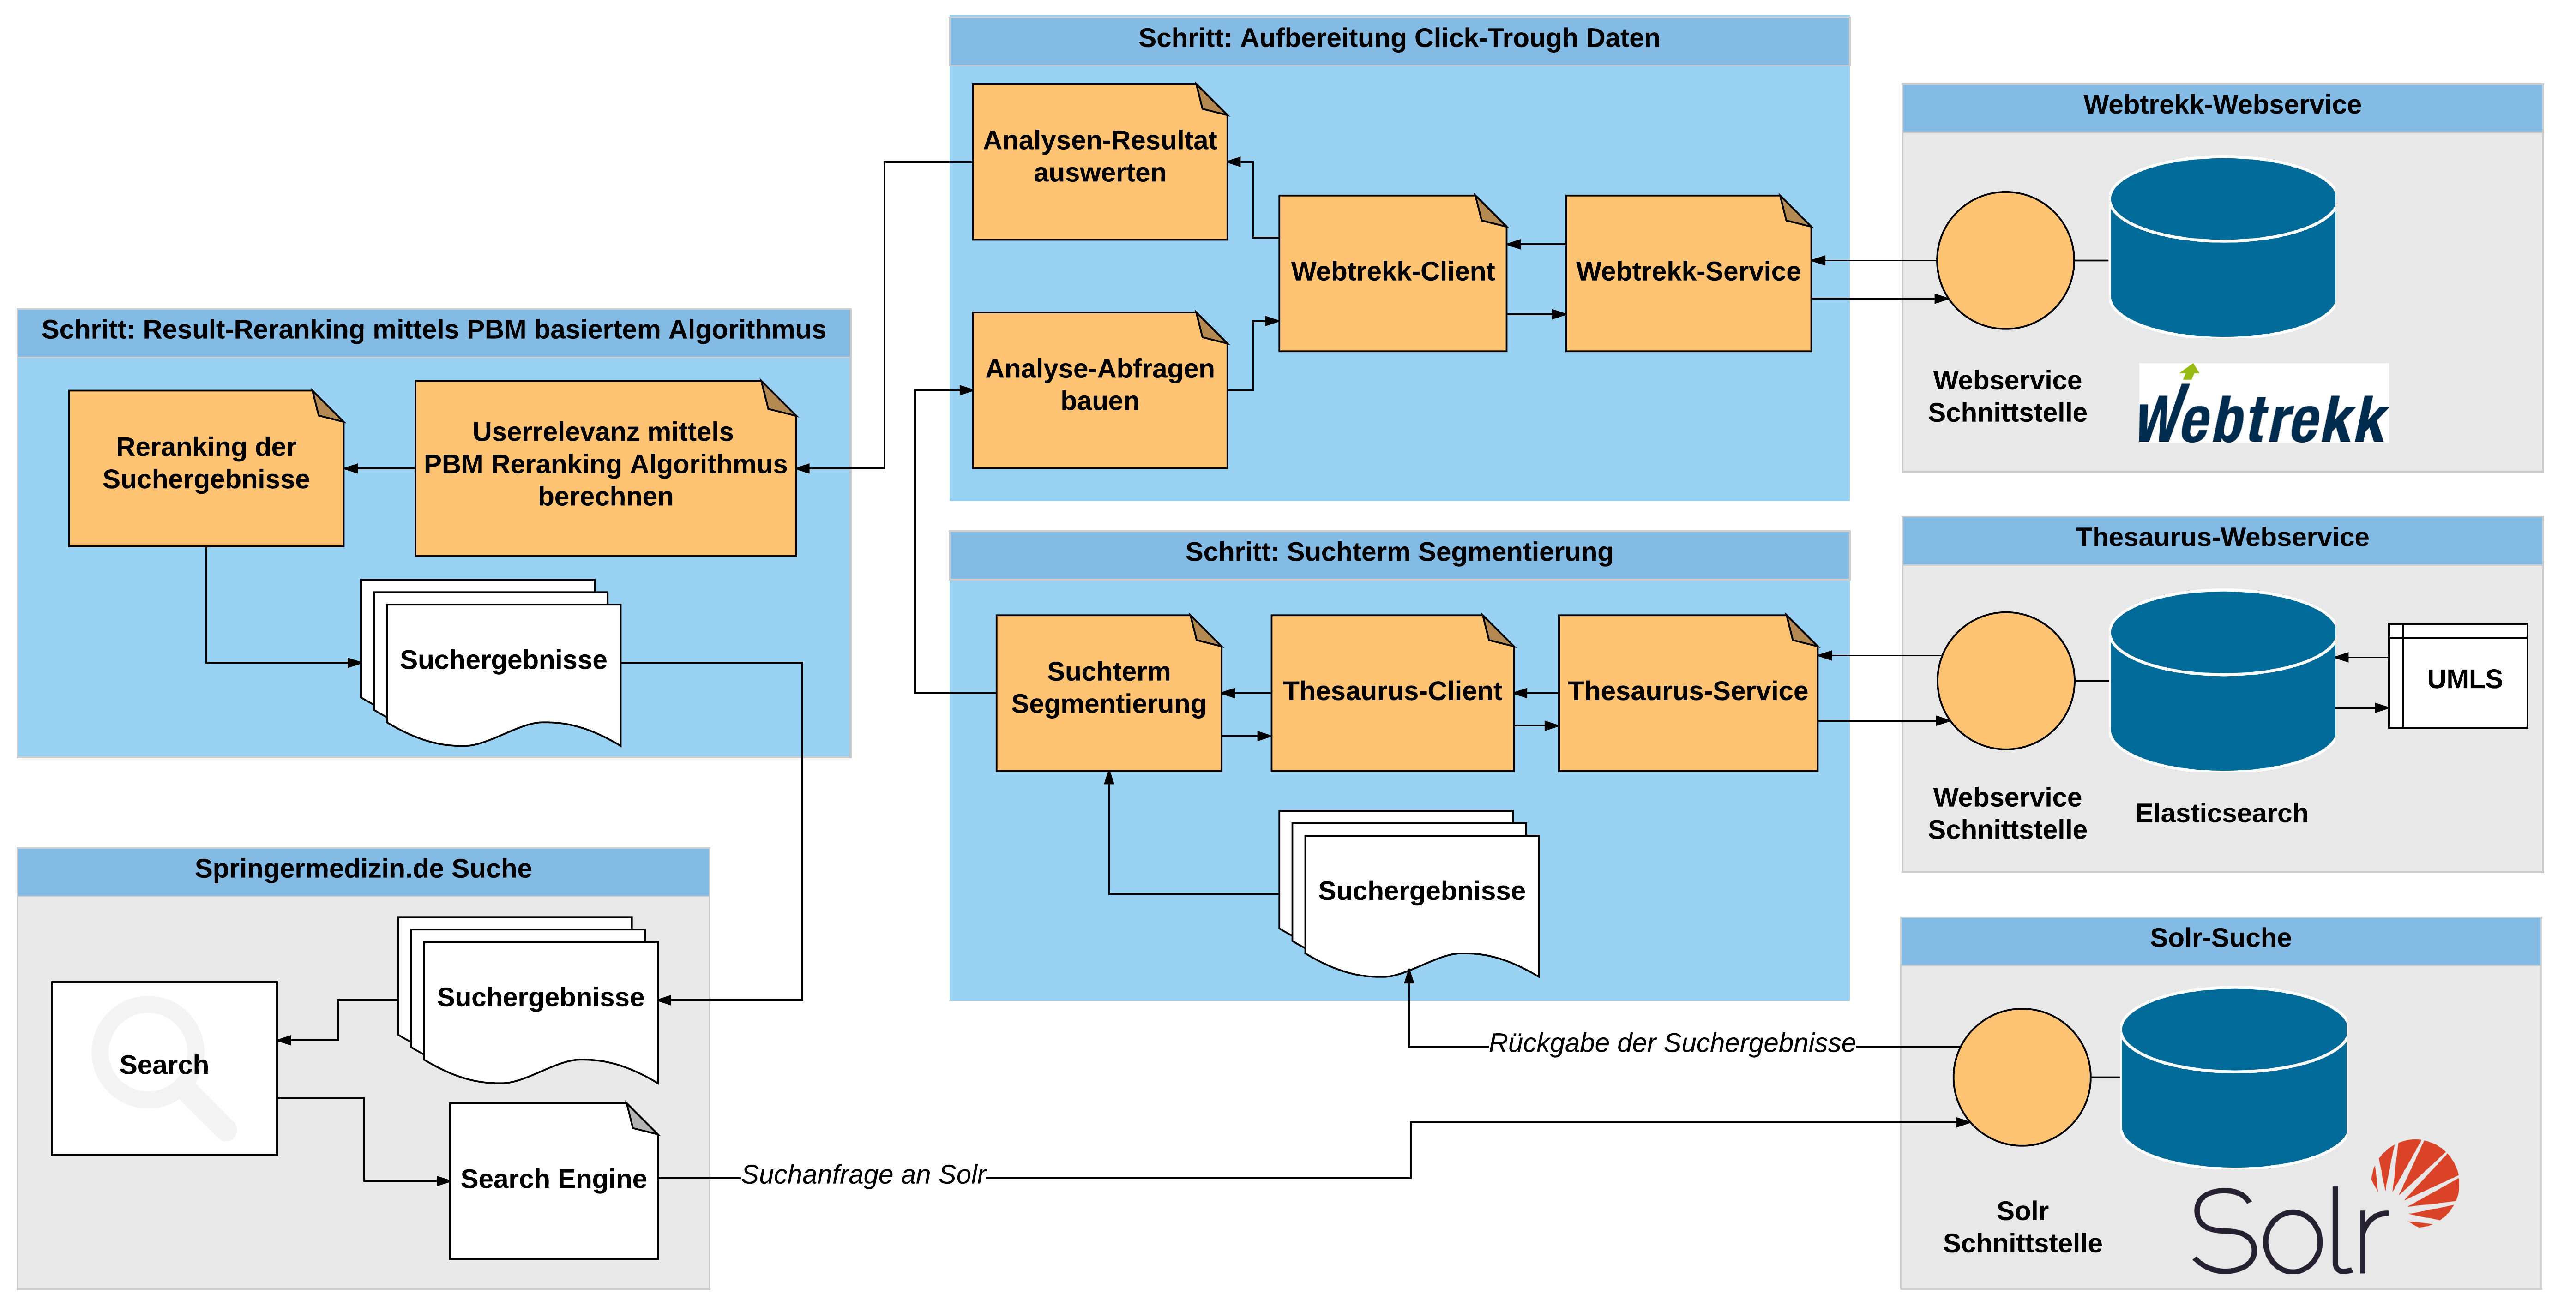
\includegraphics[width=\linewidth]{gfx/ImplementierungProzessbild}
\vspace{-2.5em}
\end{figure}

Wie bereits in Kapitel \ref{sec:Grundlagen:Grundbegriffe:Result-RerankingPBM:AnsatzSucheEinbinden} angesprochen, binden wir den Algorithmus als ein, in sich geschlossenes, unabhängiges Modul zwischen dem Suchprozess und der Aufbereitung des Suchresultats ein. Wie wir in der Abbildung sehen können, wird zuerst der Suchvorgang auf der Solr durchgeführt, bevor wir die Suchergebnisliste entgegennehmen, verarbeiten und mit unserem Reranking-Algorithmus neu sortieren. Die daraus resultierende Ergebnisliste geben dann der Suche als Suchresultat zurück. 

\section{Highlight: PBM basierter Reranking-Algorithmus}
\label{sec:Implementierung:PBM}

Der grafisch dargestellte Prozess in Abb. \ref{fig:ProzessbildImplementierung} entspricht hier nicht nicht der Reihenfolge, wie die Komponenten in der Suche aufgerufen werden, sondern der Reihenfolge der Verarbeitungsschritte im Prozess. In der effektiven Implementierung, übernimmt die Reranking-Komponente die Koordination der Verarbeitungsschritte. Sie wird im Suchprozess direkt \textit{vor der Aufbereitung} der Suchergebnisse aufgerufen und nimmt die Liste der Suchergebnisse der Solr entgegen. Sind alle Schritte des Reranking-Algorithmus verarbeitet, gibt die Reranking-Komponente die \textit{neu sortierte Liste} der Suchergebnisse zurück. Diese wird dann wieder von der Springermedizin-Suche für die Ausgabe als Suchergebnisse aufbereitet.

\subsubsection{Pseudo-Code der Reranking-Komponente}
\label{sec:Implementierung:PBM:Pseudocode}

Um den angesprochenen Vorgang des Rerankings der Suchergebnisse besser zu verstehen, sehen wir hier folgend den Programm-Ablauf der Reranking-Komponente als Pseudo-Code beschrieben:

\begin{figure}[H]
\centering
\vspace{-1em}
\caption[Pseudcode Reranking-Algorithmus]{Pseudcode Reranking-Algorithmus}
\label{fig:PseudcodeRerankingAlgorithmus}
\vspace{.5em}
\DontPrintSemicolon
\begin{algorithm}[H]
\caption{PBM basierter Reranking-Algorithmus}
\BlankLine
\Daten{$searchTerm$ (Suchterm der Suchanfrage), $searchResult$ (zu verarbeitende Suchergebnisliste)}
\Ergebnis{$rerankedSearchResult \leftarrow$ durch Reranking-Algorithmus sortierte Suchergebnisliste}
\BlankLine

\Begin{
	$keywords \leftarrow$ Segmentiere und erweitere Suchterm mittels Thesaurus\;
	$ctrClickDataBySearchTerm \leftarrow$  Lese Click-Through-Daten aus Webtrekk mithilfe von $keywords$\;

	\BlankLine
	\eIf{$ctrClickDataBySearchTerm$ ist gefüllt}{
		\BlankLine
		$ranks \leftarrow$ Lese die angeklickten Positionen aus  $ctrClickDataBySearchTerm$\;
		$ctrClickDataByRanks \leftarrow$ Lese Click-Through-Daten aus Webtrekk mithilfe von $ranks$\;
		
		\BlankLine
		\eIf{$ctrClickDataByRanks$ ist gefüllt}{
			\BlankLine
			\tcc{Berechne Klick-Wahrscheinlichkeit $P(C_{u})$ aller Dokumente $u$}
			\For{ $u \in searchResult$}{
				$\lambda \leftarrow$ Definiere $\lambda$ anhand des vordefinierten Gewichtungsfaktors für die Position $r$ des Dokumentes $u$\;
				$P(E_{r_{u}}) \leftarrow$ Berechne Klick-Wahrscheinlichkeit für Position $r$ des Dokumentes $u$\;
				$P(A_{u}) \leftarrow$ Berechne Klick-Wahrscheinlichkeit für Dokument $u$ zu Suchterm $searchTerm$\;
				\BlankLine
    			$P(C_{u}) \leftarrow \lambda\cdot P(E_{r_{u}}) + (1 - \lambda)\cdot P(A_{u})$\; 
			}
			$ranksByClickProbability \leftarrow$ Sortiere Liste $searchResult$ anhand der $P(C_{u})$ Werte
			
			\BlankLine
			\tcc{Berechne Zufallswert $X_{u}$ aller Dokumente $u$}
			\For{ $u \in searchResult$}{
    			$X_{u} \leftarrow$ Berechne Zufallswert zwischen 1 und $maxPosition(searchResult)$\; 
			}
			$ranksByRandomValue \leftarrow$ Sortiere Liste $searchResult$ anhand der $X_{u}$ Werte
			
			\BlankLine
			\tcc{Berechne effektiven Relevanz-Wert $R_{u}$ aller Dokumente $u$}
			\For{ $u \in searchResult$}{
				$\lambda \leftarrow$ Definiere $\lambda$ anhand des vordefinierten Gewichtungsfaktors für den Zufallswert $X_{u}$\;
				$r_{P(C_{u})} \leftarrow$ Lese Position des Wahrscheinlichkeits-Wertes $P(C_{u})$ aus $ranksByClickProbability$\;
				$r_{X_{u}} \leftarrow$ Lese Position des Zufallswertes $X_{u}$ aus $ranksByRandomValue$\;
				\BlankLine
    			$R_{u} \leftarrow 1 / \left(\lambda\cdot r_{X_{u}} + (1 - \lambda)\cdot r_{P(C_{u})}\right)$\;
			}
			$rerankedSearchResult \leftarrow$ Sortiere Liste $searchResult$ anhand der $R_{u}$ Werte\;
			\tcc{Rückgabe der durch den Reranking-Algorithmus umsortierten Suchergebnisse}
			\KwRet{die ersten 20 Elemente von $rerankedSearchResult$}
		}{	
			\tcc{Keine Click-Through-Daten für die angeklickten Positionen gefunden $\Rightarrow$\\
			Keine Umsortierung der Suchergebnisse mit Reranking-Algorithmus}
			\KwRet{die ersten 20 Elemente von $searchResult$}
		}
	}{
		\tcc{Keine Click-Through-Daten für Suchterm gefunden $\Rightarrow$\\
		Keine Umsortierung der Suchergebnisse mit Reranking-Algorithmus}
		\KwRet{die ersten 20 Elemente von $searchResult$}
	}
}
\end{algorithm}
\end{figure}

\section{Highlight: Webtrekk-Analysen}
\label{sec:Implementierung:Webtrekk}

Wie in der Einführung dieser Arbeit in \ref{sec:Einfuehrung:AufbauSucheBeiSpringerNature:Webtrekk} angesprochen, speichert Springermedizin seine Tracking-Daten auf Webtrekk. Für die Implementierung des Reranking-Algorithmus müssen wir die Click-Trough-Daten für die Wahrscheinlichkeits-Berechnungen, wie in \ref{sec:Reranking:Methodik:Result-RerankingPBM} besprochen, mithilfe von Analysen aus Webtrekk abfragen und auswerten. Wie wir diese Analysen abfragen, sehen wir folgend.

\subsubsection{Abfrage von Analysen}
\label{sec:Implementierung:Webtrekk:AnalysenAbfragen}

Der Webservice von Webtrekk bietet verschiedene Schnittstellenmethoden zum Export und Herunterladen der Tracking-Daten an. Die für uns relevante Schnittstellenmethode lautet \textit{getAnalysisData}. Mithilfe dieser Methode können die Daten der verschiedenen Analysen per REST-Schnittstelle\footnote{Representational State Transfer, ist ein Architekturmodell mit dem Webservices mit den Standard-HTTP-Methoden (GET, POST, PUT und DELETE) realisiert werden können} abgerufen werden. Um zu definieren, welche Analyse und mit welchen Filtern diese Analyse abgefragt werden soll, müssen wir folgende Parameter der Methode mitgeben: 

\textbf{Request:} \textit{Springermedizin-Suche $\rightarrow$ Webtrekk REST-Webservice}

\begin{table}[H]
\centering
\vspace{-.75em}
\caption[Beschreibung Analyse-Aufbau Webtrekk-Schnittstelle]{Beschreibung Analyse-Aufbau Webtrekk-Schnittstelle}
\vspace{-.5em}
\label{tab:BeispielCTDaten}
\footnotesize
\renewcommand*{\arraystretch}{1.2}
\resizebox{\textwidth}{!}{%
\begin{tabular}{ll}
\hline
\textbf{Parameter}   & \textbf{Beschreibung}                                                                              \\ \hline
\textit{analysis}    & Gewünschte Analyse (alle Analysen der Weboberfläche von Webtrekk sind so abrufbar)                  \\
\textit{time\_start} & Startzeit des Analysezeitraumes                                                                    \\
\textit{time\_stop}  & Stopzeit des Analysezeitraumes                                                                     \\
\textit{column}               & Ausgabe bestimmter, in der Standard-Analyse nicht vorhandener Datenspalten                           \\
\textit{analysis\_filter}     & Komplexe Filter bestehen aus einem oder mehreren Filtern, die logisch miteinander verknüpft werden \\ \hline
\end{tabular}
}
\vspace{-2em}
\end{table}

Zur Berechnung der Klick-Wahrscheinlichkeiten benötigen wir zwei verschieden Analysen. Beispiel-Anfragen für diese beiden Analysen sehen wie folgt aus:

\textbf{Suchanfrage:} \textit{Krebs $\rightarrow$ Springermedizin-Suche}

\begin{table}[H]
\centering
\vspace{-.75em}
\caption[Beispiel Analyse-Aufbau Webtrekk-Schnittstelle]{Beispiel Analyse-Aufbau Webtrekk-Schnittstelle}
\vspace{-.5em}
\label{tab:BeispielCTDaten}
\footnotesize
\renewcommand*{\arraystretch}{1.2}
\resizebox{\textwidth}{!}{%
\begin{tabular}{lll}
\hline
\textbf{Parameter}        & \textbf{Wahrscheinlichkeit $P(A_{u})$}                                                                                                                                                            & \textbf{Wahrscheinlichkeit $P(E_{r_{u}})$}                                                                                                                              \\ \hline
\textit{analysis}         & Navigation|Events                                                                                                                                                                                & Navigation|Events                                                                                                                                                      \\ \hline
\textit{time\_start}      & 2016-08-01                                                                                                                                                                                       & 2016-08-01                                                                                                                                                             \\ \hline
\textit{time\_stop}       & 2016-08-31                                                                                                                                                                                       & 2016-08-31                                                                                                                                                             \\ \hline
\textit{column}           & {[}Page Impressions,\% Visits,Ø - Suchtreffer{]}                                                                                                                                                 & {[}Page Impressions,\% Visits,Ø - Suchtreffer{]}                                                                                                                       \\ \hline
\textit{analysis\_filter} & \begin{tabular}[c]{@{}l@{}}{[} {[},Events,LIKE,searchresult-*{]},\\ {[}AND,Internal Search Phrases,LIKE,*Krebs*{]},\\ {[}OR,Internal Search Phrases,LIKE,*Maligne Tumoren*{]} {]}\end{tabular} & \begin{tabular}[c]{@{}l@{}}{[} {[},Events,LIKE,searchresult-1.*{]},\\ {[}OR,Events,LIKE,searchresult-4.*{]},\\ {[}OR,Events,LIKE,searchresult-29.*{]} {]}\end{tabular} \\ \hline
\end{tabular}
}
\vspace{-2em}
\end{table}

In der Antwort für diese Analysen werden die Click-Trough-Daten als JSON-Array\footnote{Die JavaScript Object Notation (JSON) ist ein kompaktes Format zum Austausch von Daten} zurückgegeben. Wie der ausgewertete JSON-Array aussehen kann, haben wir in Kapitel \ref{sec:Grundlagen:Grundbegriffe:Click-Through-Daten:AussehenClick-Through-Daten} angeschaut. 


\section{Zusammenfassung}
\label{sec:Implementierung:Zusammenfassung}

In diesem Kapitel haben wir eine Übersicht über die Architektur und die wichtigsten Highlights der Implementierung gekriegt. Wir wissen nun \textit{wie} der Lösungsansatz des Reranking-Algorithmus implementiert werden kann. Verknüpfen wir dieses Wissen mit dem aus Kapitel \ref{sec:Reranking}, könnten wir den Reranking-Algorithmus nun auch auf eine andere Suche adaptieren. Im nächsten Kapitel wollen wir nun mithilfe der implementierten Suche evaluieren, welche Verbesserung für das Qualitätsmaß der Suche von Springermedizin, der Lösungsansatz bringt. 		% INCLUDE: Kern der Implementierung
% !TEX root = ../thesis-example.tex
%
%************************************************
% Evaluation
%************************************************
\chapter{Evaluation und Auswertung}
\label{sec:Evaluation}

\section{Einführung}
\label{sec:Evaluation:Einfuehrung}

\subsubsection{Suchvarianten mithilfe eines Evaluationssystems vergleichen}
\label{sec:Evaluation:Einfuehrung:Evaluationssystems}

Das große Kernproblem der Überprüfung der Verbesserungen durch den untersuchten Lösungsansatz wird das Messen der Qualität der erzielten Suchergebnisse sein. Mithilfe einer Evaluation wollen wir messen, wie gut die Suchergebnis-Qualität der aktuellen Springermedizin-Suche im Vergleich zur im Zuge dieser Arbeit entwickelten Lösung ist.

\subsubsection{Ziel der Evaluation}
\label{sec:Evaluation:Einfuehrung:Ziel}

Die Evaluation soll Informationen darüber liefern, wie viel Verbesserung der neue Lösungsansatz bringt. Aus den Ergebnissen wollen wir erkennen, an welchen \glqq Schrauben\grqq{} etwas gedreht werden muss, damit die Suche wirklich gute Ergebnisse aus Sicht der User bringt.

\section{Aufbau der Analyse}
\label{sec:Evaluation:Aufbau}

\subsection{Datengrundlage}
\label{sec:Evaluation:Aufbau:Datengrundlage}

\subsubsection{Filterung der nutzbaren Daten mittels Cohens Kappa}
\label{sec:Evaluation:Aufbau:Datengrundlage:EvaluationsdatenFiltern}

Um die Zuverlässigkeit der Relevanzbewertungen zu messen, werden wir die gleichen Suchterme jeweils von zwei fachlichen Experten bewerten lassen. Das  meist verwendete  Maß  zur  Bewertung  der Übereinstimmungsgüte ist der \textit{Cohens Kappa Koeffizient}~(siehe \cite{Kappa}). Diese Zahl misst den  Anteil übereinstimmender Bewertungen. Hierbei können aber auch zufällige Übereinstimmungen entstehen. Der Cohens Kappa Koeffizient korrigiert das Maß an Übereinstimmung um diesen Zufallsfaktor. Anhand der Auswertungen werden wir ein Mindestmaß der Übereinstimmungsgüte definieren. Die darunter liegenden Bewertung werden wir in der Auswertung ignorieren. 

\subsection{Metrik}
\label{sec:Evaluation:Aufbau:Metrik}

\subsubsection{Evaluationsdaten mittels NDCG-Algorithmus auswerten}
\label{sec:Evaluation:Aufbau:Metrik:EvaluationsdatenNDCG}

Um das Qualitätsmaß der beiden Suchen vergleichen zu können werden wir den Bewertungsalgorithmus \textit{NDCG}~(siehe \cite{NDCG}) einsetzen. Dieser geht davon aus, dass besser positionierte Suchergebnisse eine höhere Relevanz als schlechter positionierte haben. Der NDCG vergleicht die Reihenfolge der Relevanzbewertungen der Suchergebnisse mit der idealen Reihenfolge derselben Relevanzbewertungen. Im Idealfall entspricht die Reihenfolge der Suchergebnisse der Relevanz der Suchergebnisse.

\subsubsection{Qualitätsmaß einer Suchvariante bestimmen}
\label{sec:Evaluation:Aufbau:Metrik:QualitaetMessen}

In der Evaluation werden zu jedem Suchterm zwei Bewertungen für die Springermedizin-Suche und zwei Bewertungen für die Suche mit dem hier zu untersuchenden Lösungsansatz abgegeben. Um das Qualitätsmaß einer Suchvariante zu einem Suchterm zu bestimmen, berechnen wir den NDCG der beiden Bewertungen. Nehmen wir den Mittelwert der beiden resultierenden NDCG-Werte, erhalten wir den effektiven NDCG-Wert. Die NDCG-Werte der beiden Suchen können wir dann miteinander vergleichen.

\subsection{Vorgehen}
\label{sec:Evaluation:Aufbau:Vorgehen}

\subsubsection{Evaluationssystem aufbauen}
\label{sec:Evaluation:Aufbau:Vorgehen:Aufbau}

Um eine Evaluation durchführen zu können, müssen wir eine passende Testumgebung aufbauen. Diese besteht aus einem Evaluationssystem, einer Instanz der aktuellen Springermedizin-Applikation und einer Instanz des neu implementierten Lösungsansatzes. Auf dem Evaluationssystem sollen fachliche Experten (Redakteure von Springermedizin) die Relevanz der Suchergebnisse  der beiden Suchmaschinen vergleichen. Dazu sollen die jeweils besten 10 Suchergebnisse nach Relevanz zum Suchterm bewertet werden. Der Ergebnisse werden in einer Datenbank gespeichert, um sie später auszuwerten. 

\subsubsection{Evaluationssystem auswerten}
\label{sec:Evaluation:Aufbau:Vorgehen:Auswerten}

Nach Ablauf der Evaluationsphase werden wir die Evaluations-Daten auswerten. Die Auswertung der Daten findet direkt im Evaluationssystem statt. 
\\
\\
Dazu werden die Daten aus der Datenbank gelesen und mit dem Cohens Kappa Koeffizienten die nutzbaren Daten gefiltert. 

\subsection{Durchführung}
\label{sec:Evaluation:Aufbau:Durchfuehrung}

\subsubsection{Verschiedene Varianten des neuen Lösungsansatzes werden evaluiert}
\label{sec:Evaluation:Aufbau:Durchfuehrung:EvaluationsdatenVarianteLoesungsansatzes}

Der in dieser Arbeit zu untersuchende Lösungsansatz kann verschieden konfiguriert werden. Wir können den Einfluss des Zufallsfaktors bestimmen. Um verschiedene Konstellationen testen zu können, werden wir mit zwei verschiedenen Werten für den Einfluss des Zufallsfaktor evaluieren. Die Click-Trough-Daten von an der Applikation angemeldeten Benutzern können wir von den Click-Trough-Daten von anonymen Benutzern unterscheiden.
\\
\\
Aus den beiden Einflusswerten des Zufallsfaktors und der Unterscheidung zwischen angemeldeten und anonymen Benutzern, ergeben sich vier Konstellationen, die evaluiert werden können. Jeder Konstellation werden wir jeweils 25 Prozent der Suchterme zuteilen. Mithilfe des Evaluationssystems werden wir die Zuteilung der Suchterme zufällig generieren lassen.
\\
\\
Hier folgend die Aufteilung der generierten Analysen:

\centering
\begin{myitemize}
\setlength\itemsep{0em}
\item Springermedizin.de Suche 
\begin{myitemize}
\item 50\% der Analysen
\end{myitemize}
\end{myitemize}
\begin{myitemize}
\item Reranking Suche 
\begin{myitemize}
\item 50\% der Analysen
\begin{myitemize}
\item Einfluss Zufallsranking 0.1: 25\% der Analysen 
\end{myitemize}
\begin{myitemize}
\item Einfluss Zufallsranking 0.01: 25\% der Analysen 
\end{myitemize}
\end{myitemize}
\end{myitemize}

\section{Auswertung der Suchergebnis-Qualität}
\label{sec:Evaluation:Auswertung}

\subsection{Quantitative Auswertung}
\label{sec:Evaluation:Auswertung:QuantitativeAuswertung}

\subsection{Diskussion}
\label{sec:Evaluation:Auswertung:Diskussion}

\section{Zusammenfassung}
\label{sec:Evaluation:Zusammenfassung}			% INCLUDE: Evaluation
% !TEX root = ../thesis-example.tex
%
%************************************************
% Zusammenfassung und Ausblick
%************************************************
\chapter{Zusammenfassung und Ausblick}
\label{sec:ZusammenfassungAusblick}

\section{Zusammenfassung}
\label{sec:ZusammenfassungAusblick:Zusammenfassung}

\section{Ausblick}
\label{sec:ZusammenfassungAusblick:Ausblick} 		% INCLUDE: Zusammenfassung

\pagebreak

%************************************************
% Anhang
%************************************************
% !TEX root = ../thesis-example.tex
%
%************************************************
% Anhang
%************************************************
\chapter{Anhang}
\label{sec:Anhang}

\section{Verwendete Suchterme für die Evaluation}
\label{sec:Anhang:VerwendeteSuchtermeEvaluation}

\begin{table}[H]
\centering
\vspace{-.5em}
\caption[Tabelle der verwendeten Suchterme für die Evaluation]{Tabelle der verwendeten Suchterme für die Evaluation}
\label{tab:TabelleSuchtermeEvaluation}
\vspace{-.5em}
\small
\renewcommand*{\arraystretch}{1.2}
\resizebox{\textwidth}{!}{%
\begin{tabular}{ll|ll}
\hline
\textbf{Fachgebiet}                             & \textbf{Suchphrasen}                          & \textbf{Fachgebiet}                                           & \textbf{Suchphrasen}         \\ \hline
\multirow{10}{*}{\textit{\textbf{Onkologie}}}   & pankreaskarzinom                              & \multirow{10}{*}{\textit{\textbf{AINS}}}                      & Borreliose                   \\
                                                & schilddrüsenkarzinom                          &                                                               & myokarditis                  \\
                                                & ernährung onkologie                           &                                                               & herzinsuffizienz             \\
                                                & plasmozytom                                   &                                                               & adipositas                   \\
                                                & thyreoidektomie                               &                                                               & gastrointestinale blutung    \\
                                                & magenkarzinom                                 &                                                               & helicobacter pylori          \\
                                                & rektumkarzinom radiochemotherapie             &                                                               & diabetes mellitus            \\
                                                & operative therapie                            &                                                               & stroke                       \\
                                                & Prostata-Adenom                               &                                                               & darmatonie                   \\
                                                & lebermetastasen                               &                                                               & herpes zoster                \\ \hline
\multirow{20}{*}{\textit{\textbf{Zahnmedizin}}} & mandibular advancement device                 & \multirow{10}{*}{\textit{\textbf{Neurologie, Psychiatrie}}}   & schlaganfall                 \\
                                                & fibrinogen                                    &                                                               & demenz                       \\
                                                & lidocain                                      &                                                               & schlafstörungen              \\
                                                & therapietreue                                 &                                                               & delir                        \\
                                                & Berufsdermatologie                            &                                                               & virusenzephalitis            \\
                                                & trigeminusneuralgie                           &                                                               & invagination                 \\
                                                & anaphylaxie                                   &                                                               & adhs                         \\
                                                & konservative therapie                         &                                                               & demenz therapie              \\
                                                & mukositis                                     &                                                               & psychiatrische erkrankungen  \\
                                                & kraniofaziale chirurgie                       &                                                               & syringomyelie                \\ \cline{3-4} 
                                                & versiegelung zähne                            & \multirow{10}{*}{\textit{\textbf{Innere Medizin}}}            & hyponatriämie                \\
                                                & präoperative aufklärung                       &                                                               & osteoporose                  \\
                                                & antibiotika                                   &                                                               & copd                         \\
                                                & hiv-infektion                                 &                                                               & sarkoidose                   \\
                                                & implantatallergie                             &                                                               & vorhofflimmern               \\
                                                & patientenakte                                 &                                                               & tuberkulose                  \\
                                                & blutung postoperativ                          &                                                               & migration                    \\
                                                & disposition                                   &                                                               & lungenembolie                \\
                                                & überempfindlichkeit                           &                                                               & betablocker                  \\
                                                & schweigepflicht                               &                                                               & das fiebernde kleinkind      \\ \hline
\multirow{10}{*}{\textit{\textbf{Gynäkologie}}} & reproduktion                                  & \multirow{10}{*}{\textit{\textbf{Orthopädie, Urologie, HNO}}} & talusfrakturen               \\
                                                & konisation                                    &                                                               & mediale schenkelhalsfraktur  \\
                                                & impfen in der schwangerschaft                 &                                                               & winkelstabile osteosynthese  \\
                                                & schwangerschaft melisse                       &                                                               & chronische rhinosinusitis    \\
                                                & risikoschwangerschaft                         &                                                               & urethralsyndrom              \\
                                                & sectio cesarea                                &                                                               & nacken schmerzen             \\
                                                & adenoviren neonatal                           &                                                               & implantierbare hörgeräte     \\
                                                & mammakarzinom                                 &                                                               & schmerzen an der wirbelsäule \\
                                                & sexuelle gewalt spurensicherung dokumentation &                                                               & ac gelenk                    \\
                                                & frühschwangerschaft                           &                                                               & basaliom                     \\ \hline
\end{tabular}
}
\end{table}

\pagebreak

\cleardoublepage

\addtocontents{toc}{\vspace{\normalbaselineskip}}

\addcontentsline{toc}{section}{Literatur-Verzeichnis}
{%
\setstretch{1.1}
\renewcommand{\bibfont}{\normalfont\small}
\setlength{\biblabelsep}{0pt}
\setlength{\bibitemsep}{0.5\baselineskip plus 0.5\baselineskip}
\printbibliography[nottype=online]
\printbibliography[heading=subbibliography,title={Webseiten},type=online,prefixnumbers={@}]
}
\cleardoublepage

\addcontentsline{toc}{section}{Abbildungs-Verzeichnis}
\listoffigures
\cleardoublepage

\addcontentsline{toc}{section}{Tabellen-Verzeichnis}
\listoftables
\cleardoublepage 			% INCLUDE: Anhang

% **************************************************
% End of Document CONTENT
% **************************************************
\end{document}
